\documentclass [11pt,twoside]{article}
\usepackage[utf8]{inputenc}
\usepackage[T1]{fontenc}

%Page margins, header and footer positions
\usepackage{geometry}
 \geometry{
 a4paper,
 total={210mm,297mm},
 left=25mm,
 right=25mm,
 top=30mm,
 bottom=25mm,
 headsep=7mm}

\interfootnotelinepenalty=10000

%To display filling dots in the TOC for all entries
\usepackage[titles]{tocloft}
\renewcommand{\cftsecleader}{\cftdotfill{\cftdotsep}}

%Define new header and footer style
\usepackage{fancyhdr}

\pagestyle{fancy}
\fancyhf{}
\lhead{\color{Gray}{\small{Travlendar+ project by YOUR NAMES}}}
\lfoot{\textcolor{Gray}{\small{Copyright © 2017, YOUR NAMES – All rights reserved}}}
\rfoot{\textcolor{Gray}{\thepage}}
\renewcommand{\headrulewidth}{0pt}

%PACKAGES
\usepackage{wasysym}
\usepackage{pifont}

\newcommand{\supported}{\ding{52}\xspace}
\newcommand{\unsupported}{\ding{55}\xspace}
\newcommand{\partsupported}{\textcolor{black!40}{\ding{52}}\xspace}
\newcommand{\lowsupported}{\textcolor{black!20}{\ding{52}}\xspace}
\newcommand{\unknowsupported}{\textbf{?}\xspace}

%Font: Times
\usepackage{times}
%Change monospaced font
\renewcommand{\ttdefault}{lmtt}

%tables
\usepackage{tabu}
\usepackage{tabularx}
\usepackage{ltablex}
\usepackage{longtable}
\usepackage{float} % To allow the use of H modifier in long tables

%landscape mode
\usepackage{pdflscape}
\usepackage{rotating}
\usepackage{caption}

%make landscape mode be sensitive to even and odd pages
%start
\def\myrotate{\ifodd\c@page\else-\fi 90}
\makeatletter
\global\let\orig@begin@landscape=\landscape%
\global\let\orig@end@landscape=\endlandscape%
\gdef\@true{1}
\gdef\@false{0}
\gdef\landscape{%
    \global\let\within@landscape=\@true%
    \orig@begin@landscape%
}%
\gdef\endlandscape{%
    \orig@end@landscape%
    \global\let\within@landscape=\@false%
}%
\@ifpackageloaded{pdflscape}{%
    \gdef\pdf@landscape@rotate{\PLS@Rotate}%
}{
    \gdef\pdf@landscape@rotate#1{}%
}
\let\latex@outputpage\@outputpage
\def\@outputpage{
    \ifx\within@landscape\@true%
        \if@twoside%
            \ifodd\c@page%
                \gdef\LS@rot{\setbox\@outputbox\vbox{%
                    \pdf@landscape@rotate{-90}%
                    \hbox{\rotatebox{90}{\hbox{\rotatebox{180}{\box\@outputbox}}}}}%
                }%
            \else%
                \gdef\LS@rot{\setbox\@outputbox\vbox{%
                    \pdf@landscape@rotate{+90}%
                    \hbox{\rotatebox{90}{\hbox{\rotatebox{0}{\box\@outputbox}}}}}%
                }%
            \fi%
        \else%
            \gdef\LS@rot{\setbox\@outputbox\vbox{%
                \pdf@landscape@rotate{+90}%
                \hbox{\rotatebox{90}{\hbox{\rotatebox{0}{\box\@outputbox}}}}}%
            }%
        \fi%
    \fi%
    \latex@outputpage%
}
\makeatother
%end

%graphics
\usepackage{graphicx}
\usepackage[dvipsnames, table]{xcolor}
%If you upload images from PC, you need to insert code for the path here (different for Windows and Unix OS)

%References
%\usepackage{xpatch}
%\usepackage[backend=biber, style=numeric, citestyle=numeric, sorting=none]{biblatex}
%\addbibresource{main.bib}

%Other
\usepackage{ifthen}
\usepackage{xspace}
\usepackage{enumitem}
\usepackage{amssymb}
\usepackage[pdftex, colorlinks]{hyperref}
\newcommand{\comment}[1]{{\color{Red}$\blacktriangleright$ Comment: #1 $\blacktriangleleft$}}


% Some utilities\ldots
\usepackage{soul}
\usepackage{tikz}

\usetikzlibrary{calc}
\usetikzlibrary{decorations.pathmorphing}


\makeatletter

\newcommand{\defhighlighter}[3][]{%
  \tikzset{every highlighter/.style={color=#2, fill opacity=#3, #1}}%
}

\defhighlighter{yellow}{.5}

\newcommand{\highlight@DoHighlight}{
  \fill [ decoration = {random steps, amplitude=1pt, segment length=15pt}
        , outer sep = -15pt, inner sep = 0pt, decorate
       , every highlighter, this highlighter ]
        ($(begin highlight)+(0,8pt)$) rectangle ($(end highlight)+(0,-3pt)$) ;
}

\newcommand{\highlight@BeginHighlight}{
  \coordinate (begin highlight) at (0,0) ;
}

\newcommand{\highlight@EndHighlight}{
  \coordinate (end highlight) at (0,0) ;
}

\newdimen\highlight@previous
\newdimen\highlight@current

\DeclareRobustCommand*\highlight[1][]{%
  \tikzset{this highlighter/.style={#1}}%
  \SOUL@setup
  %
  \def\SOUL@preamble{%
    \begin{tikzpicture}[overlay, remember picture]
      \highlight@BeginHighlight
      \highlight@EndHighlight
    \end{tikzpicture}%
  }%
  %
  \def\SOUL@postamble{%
    \begin{tikzpicture}[overlay, remember picture]
      \highlight@EndHighlight
      \highlight@DoHighlight
    \end{tikzpicture}%
  }%
  %
  \def\SOUL@everyhyphen{%
    \discretionary{%
      \SOUL@setkern\SOUL@hyphkern
      \SOUL@sethyphenchar
      \tikz[overlay, remember picture] \highlight@EndHighlight ;%
    }{%
    }{%
      \SOUL@setkern\SOUL@charkern
    }%
  }%
  %
  \def\SOUL@everyexhyphen##1{%
    \SOUL@setkern\SOUL@hyphkern
    \hbox{##1}%
    \discretionary{%
      \tikz[overlay, remember picture] \highlight@EndHighlight ;%
    }{%
    }{%
      \SOUL@setkern\SOUL@charkern
    }%
  }%
  %
  \def\SOUL@everysyllable{%
    \begin{tikzpicture}[overlay, remember picture]
      \path let \p0 = (begin highlight), \p1 = (0,0) in \pgfextra
        \global\highlight@previous=\y0
        \global\highlight@current =\y1
      \endpgfextra (0,0) ;
      \ifdim\highlight@current < \highlight@previous
        \highlight@DoHighlight
        \highlight@BeginHighlight
      \fi
    \end{tikzpicture}%
    \the\SOUL@syllable
    \tikz[overlay, remember picture] \highlight@EndHighlight ;%
  }%
  \SOUL@
}

\makeatother

% Common abbrev. are set as commands to ensure proper spacing after the dot
\RequirePackage{xspace}
\newcommand{\ie}{i.e.\@\xspace}
\newcommand{\aka}{a.k.a.\@\xspace}
\newcommand{\Ie}{I.e.\@\xspace}
\newcommand{\cf}{cf.\@\xspace}
\newcommand{\Cf}{Cf.\@\xspace}
\newcommand{\eg}{e.g.\@\xspace}
\newcommand{\Eg}{E.g.\@\xspace}
\newcommand{\etal}{et al.\@\xspace}
\newcommand{\etc}{etc.\@\xspace}
\newcommand{\wrt}{w.r.t.\@\xspace}
\newcommand{\Wrt}{W.r.t.\@\xspace}



\date{}


\begin{document}

%TITLE PAGE

\begin{titlepage}


%LOGO

{\begin{table}[t!]
\centering
\begin{tabu} to \textwidth { X[1.3,r,p] X[1.7,l,p] }
\textcolor{Blue}
{\textbf{\small{Travlendar+ project YOUR NAMES}}} & 
\includegraphics[scale=0.5]{Images/PolimiLogo}
\end{tabu}
\end{table}}~\\ [7cm]

%TITLE 

\begin{flushleft}

%Replace the text string with your title
{\textcolor{Blue}{\textbf{\Huge{Requirement Analysis and Specification
        Document}}}} \\ [1cm]

\end{flushleft}

\end{titlepage}

%Define deliverable specific info
%Replace cell contents where needed
\begin{table}[h!]
\begin{tabu} to \textwidth { X[0.3,r,p] X[0.7,l,p] }
\hline

\textbf{Deliverable:} & RASD\\
\textbf{Title:} & Requirement Analysis and Verification Document \\
\textbf{Authors:} & YOUR NAMES \\
\textbf{Version:} & 1.0 \\ 
\textbf{Date:} & 31-January-2016 \\
\textbf{Download page:} & LINK TO YOUR REPOSITORY \\
\textbf{Copyright:} & Copyright © 2017, YOUR NAMES – All rights reserved \\
\hline
\end{tabu}
\end{table}




\setcounter{page}{2}


%------------------------------------------------------------------------------------------------------------------------------------------------
\newpage
\addcontentsline{toc}{section}{Table of Contents}
\tableofcontents
\newpage
\addcontentsline{toc}{section}{List of Figures}
\listoffigures
\addcontentsline{toc}{section}{List of Tables}
\listoftables

%------------------------------------------------------------------------------------------------------------------------------------------------
\clearpage
{\color{Blue}{\section{Introduction}}}
\label{sect:introduction}
\subsection{Scope}
Traditional software programming education often lacks of hands-on experience and continuous evaluation. CodeKataBattle addresses these issues by providing a platform for competitive programming challenges which promotes teamwork and emphasizes the test-first approach in software development. It allows students to apply theoretical knowledge in tournaments with an automated scoring system. Instructors benefit from closer mentorship through code reviews and manual evaluation, creating a cycle of learning through practice, feedback, and community engagement.
\\\\CodeKataBattle's platform will employ a microservices architecture, emphasizing the decomposition of the system into small, independently deployable services. Each microservice will be dedicated to a specific business capability, promoting modular development and ease of maintenance.The architecture facilitates scalability, allowing individual services to be scaled independently based on demand.
Other important design choices include:
\begin{itemize}
    \item \textbf{Service Discovery}: A service registry will be used to allow services to locate each other without prior knowledge of their location. This enables efficient communication between services by providing up-to-date information. Service discovery enhances fault tolerance and load balancing, contributing to the overall reliability of the system.
    \item \textbf{API Gateway}: An API gateway will be used to provide a single entry point for clients to access the system. This simplifies the client interface by abstracting the underlying microservices and provides a centralized location for authentication and authorization. The API Gateway enhances security measures, ensuring controlled and secure access to the microservices.
    \item \textbf{Hybrid Communication Framework}: While most services exploit synchronous communication via REST api calls, an event-driven communication framework is also used to facilitate communication between specific microservices, allowing them to be loosely coupled and promoting both modularity and scalability. This framework enhances the reliability of these services by providing a mechanism for asynchronous communication between them (i.e. queues).
    \item \textbf{Data Management Strategies}: The system employs tailored data management strategies, utilizing databases suitable for microservices. Both relational and NoSQL databases are considered for each specific service in order to provide flexibility and scalability.
\end{itemize}
Incorporating these key properties into the CodeKataBattle system should provide a robust and scalable architecture, ensuring modularity, responsiveness, security, reliability, and effective data management.

\subsection{Definitions, Acronyms, Abbreviations}
TODO: remove unused ones
\subsubsection{Definitions}
\begin{itemize}
    \item {\textbf{User:} anyone that has registered to the platform}
    \item {\textbf{Student:} the first kind of users and, basically, the people this product is designed for. Their objective is to submit solutions to battles}
    \item {\textbf{Team:} students can decide to group up and form a team to partecipate to a battle. The score assigned to the submission of a team will be assigned also to each one of its members}
    \item {\textbf{Educator:} the second kind of users. They create tournaments, set-up battles, and eventually, evaluate the solutions that teams of students have submitted during the challenge}
    \item {\textbf{Tournament:} collection of coding exercises (battles) about specific topics of a subject. Interested students can subscribe to it and participate to its battles as soon as they are published}
    \item {\textbf{Code Kata Battle (or battle):} the atomic unit of a tournament. Usually students are asked to implement an algorithm or to develope a simple project that solves the task. Each battle belongs to a specific tournament: students submitting solutions for a battle will obtain a score that will be used to compute both the team's rank for the battle and the members' tournament rank}
    \item {\textbf{Code Kata:} description and software project necessary for the battle, including test cases and build automation scripts. These are uploaded by the educator at battle creation time}
    \item {\textbf{Tournament collaborator:} other educator that is added by the tournament creator to help him in the management of the tournament. He can create battles and evaluate their submissions}
    \item {\textbf{GitHub:} web-based hosting service for version control, mostly used for computer code. It offers both distributed version control and source code management functionalities}
    \item {\textbf{GitHub repository:} a repository is a storage space where some project files are stored. It can be either public or private. In the context of the platform, each battle is associated with a GitHub repository that is created by the system and shared with the teams}
    \item {\textbf{GitHub collaborator:} person who is granted access to a GitHub repository with write permission}
    \item {\textbf{GitHub Actions:} GitHub feature that allows to automate tasks directly on GitHub, such as building and testing code, or deploying applications. In the context of the platform, GitHub Actions is used to automatically notify the system when a new submission is pushed to the repository of a team}
    \item {\textbf{Test cases:} each battle is associated with a set of test cases, which  are input-output value pairs that describe the correct behavior of the ideal solution}
    \item {\textbf{Static analysis:} is the analysis of programs performed without executing them, usually achieved by applying formal methods directly to the source code. In the context of the platform this kind of analysis is used to extract additional information about the level of security, reliability and maintainability of a battle submission}
    \item {\textbf{Functional analysis:} measures the correctness of a solution in terms of passed test cases}
    \item {\textbf{Timeliness:} measures the time passed between the start of the battle and the last commit of the submission}
    \item {\textbf{Score:} to each solution is assigned a score which is computed taking into account timeliness, functional and static analysis and, eventually, manual score assigned by the educator that created the challenge. The score is a natural number between 0 and 100 (the higher the better)}
    \item {\textbf{Rank:} during a battle, students can visualize the ranking of teams taking part to the battle. Moreover, at the end of each battle, the platform updates the personal tournament score of each student. Specifically, the score is computed as the sum of all the battles scores received in that tournament. This overall score is used to fill out a ranking of all the students participating to the tournament which is accessible by any time and by any user subscribed to the platform}
    \item {\textbf{Notification:} it's an  email alert that is sent to users to inform them that a certain event occurred such as the creation of a new tournament and battle or the publication of the final rank of a battle}
\end{itemize}
\subsubsection{Acronyms}
\begin{itemize}
    \item {\textbf{DD:} Design Document}
    \item {\textbf{RASD:} Requirements Analysis and Specification Document}
    \item {\textbf{CKB:} Code Kata Battles}
    \item {\textbf{API:} Application Programming Interface}
    \item {\textbf{UML:} Unified Modeling Language}
    \item {\textbf{HTML:} HyperText Markup Language}
    \item {\textbf{CSS:} Cascading Style Sheets}
    \item {\textbf{JSON:} JavaScript Object Notation}
    \item {\textbf{OS:} Operating System}
    \item {\textbf{REST:} REpresentational State Transfer}
    \item {\textbf{URL:} Uniform Resource Locator}
    \item {\textbf{HTTPS:} HyperText Transfer Protocol Secure}
\end{itemize}
\subsubsection{Abbreviations}
\begin{itemize}
    \item {\textbf{Gn:} Goal number “n”}
    \item {\textbf{Dn:} Domain Assumption number “n”}
    \item {\textbf{Rn:} Requirement number “n”}
    \item {\textbf{UCn:} Use Case number “n”}
\end{itemize}

\subsection{Revision History}
\begin{itemize}
    \item \today: version 1.0 (first release)
\end{itemize}

\subsection{Reference Documents}
\begin{itemize}
    \item Specification document: "Assignment RDD AY 2023-2024"
    \item DD reference template: "04e.QualitiesAndCreatingDD.pdf"
    \item UML official specification \href{https://www.omg.org/spec/UML}{https://www.omg.org/spec/UML}
    \item GitHub API official documentation: \href{https://docs.github.com/en/rest/guides/getting-started-with-the-rest-api?apiVersion=2022-11-28}{https://docs.github.com/en/rest/guides/getting-started-with-the-rest-api?apiVersion=2022-11-28}
\end{itemize}

\subsection{Document Structure}
\begin{itemize}
    \item \textbf{Section 1: Introduction}\\ In this section a general description of the document and the system to be developed is provided, also including a glossary of terms used and a list of reference documents.
    \item \textbf{Section 2: Architectural Design}\\ Here the high-level structure of the software is outlined. This includes the identification of major components, their interactions, and the overall flow of data within the system. Dependencies on external factors or third-party integrations are also detailed, offering a comprehensive view of the software's architecture.
    \item \textbf{Section 3: User Interface Design}\\ Focused on the end-user experience, this section describes the layout, interactivity, and visual elements of the software's user interface. It includes mockups of the main pages of the web application.
    \item \textbf{Section 4: Requirements Traceability}\\ Here the relation between software requirements and design elements is highlighted. This is achieved through the use of a traceability matrix.
    \item \textbf{Section 5: Implementation, Integration and Test Plan}\\ This section is a comprehensive guide that covers the main aspects of the software development lifecycle. It outlines the details of implementation and integration plan, as well as the testing strategy.
    \item \textbf{Section 6: Effort spent}\\The sixth and last chapter contains the time spent by each contributor of this document.
\end{itemize}

%------------------------------------------------------------------------------------------------------------------------------------------------
\clearpage
{\color{Blue}{\section{Overall Description}}}
\label{sect:overview}
\subsection{Product perspective}
\subsubsection{Scenarios}
\begin{enumerate}[label=\textbf{\arabic*}.]
    \item \textbf{ Educator creates a tournament}\\Alan is a university professor. He has just finished explaining a very hard topic that occupied multiple lectures. He would like to test its class about it but exams dates are far away ahead and he thinks that trying to evaluate their understanding with a quick quiz performed in class before or after his next lecture would not be a good idea given the depth of the topic. Anyway he knows of a site that allows educators to easily organize challenges to which students can take part and decides to give it a try.\\He connects to the website of the platform and signs up as an educator. After that, he navigates to the “Tournaments” section and selects the option to create a new one: inputs the name of the tournament and a deadline for the subscription. All students subscribed to the CKB platform are now notified and can join the tournament.\\Since Alan’s schedule is often very busy, he then decides to grant the permission to create battles to his teaching assistant Thomas, which has already subscribed to the platform.
    \item \textbf{ Educator creates a battle}\\Linus is a famous youtuber that publishes video courses on programming languages. He wants to increase the engagement with his subscribers, so for this reason he has already subscribed to the CKB platform and created a tournament. In his last video lecture, he has started a new playlist on Java language, explaining some basic concepts typical of object oriented programming.\\To challenge his viewers, he decides to create a new coding battle. He now connects to the website of the platform and log-ins with his credential. He clicks on the tournament called “LinusTechChallenges” he previously created and selects the option to generate a new battle. The platform then asks him to specify some settings for this specific challenge: he selects “Java” as programming language, uploads the “code kata” which includes a textual description of the challenge and all the files related to the software project like test cases and build automation scripts, selects set the minimum and maximum number of students per group, fixes the registration and final submission deadlines. Since he has many subscribers and cannot manually review every solution, he also specifies that a final manual evaluation is not needed. However, Linus decides to enable all the available aspects the static analysis should focus on (e.g. security, reliability, maintainability). At this point he confirms the creation of the battle and the system automatically notifies all the students subscribed to the tournament about the new coding battle.
    \item \textbf{ Student subscribes to a tournament}\\Mark is struggling to keep the pace of its professor’s lectures. Moreover, since his anxiety always penalizes him, he is afraid he will organize some activity in class to evaluate his knowledge about the last, complex topic. One day, while looking at the academic mail, he notices that the feared professor is contacting its students to inform them of an alternative evaluation method that would allow them to avoid part of the final exam and which involves to write code to solve problems related with the subject and compete with other students. Mark immediately decides to go for it and subscribes (as a student) to the platform indicated by the professor. Once logged in, he goes to the “Tournaments” section and selects the option to search for a specific tournament: at this point he searches the tournament by the name communicated by the professor, selects it and subscribes to it. Once a new battle will be available, he will be notified by the system. He is now ready to participate to the battles and prove what he has learned.
    \item \textbf{ Students form a team}\\Liam is a software engineer that has subscribed to CKB because a famous IT company is offering some job positions to the most talented developers discovered through the platform. For this reason, he already joined the tournament created by the company. Since the company is interested in developers with the ability to work in teams, its human resources department has set “2” as minimum number of team members for their first battle. So, Liam decides to tackle the first challenge with a trusted former university colleague of his. He navigates to the “Tournaments” section, searches and selects the ongoing tournament of the company and clicks on the first battle called “Challenge 1”. The system shows 2 options: “Create a team” and “Join a team”. Liam selects the first option and chooses a name for his team, checking the “private” flag option. The systems generates an invite code that he can now share privately to his friend in order to join the team.
    \item \textbf{ Student submits a solution}\\Jonas is subscribed to the CKB platform in order to participate in quizzes organized by his computer science professor. He is very happy with this kind of continual evaluation because it's a great way to understand those difficult concepts taught during theory classes and skip some exercises at the final written exam.\\When a new programming challenge is announced, Jonas gets excited to test his skills. He forms a team with two other classmates to collaborate on solving the exercise. After working hard to come up with a new solution, Jonas submits it to the CKB platform by committing the solution on their GitHub repository before the deadline. Jonas and his team mates have monitored their score during the whole battle, but are not satisfied with rank of their final submission computed with the automated evaluation.\\The next day, after the consolidation stage, Jonas is thrilled to see his final team rank near the top of the leaderboard! Indeed the professor liked a lot their innovative solution and decided to  reward them during the manual evaluation.
    \item \textbf{ Educator manually evaluates solutions}\\Oliver is an instructor and he is using CKB to evaluate the students enrolled in his online programming course. He enjoys the platform because it organizes the students’ GitHub repository in a convenient and central way. Indeed, once the submission phase ends, during the consolidation stage Oliver can select the current battle and go through the whole list of teams. For each team, the system shows the GitHub repository link and the scores related to the automated evaluation. After inspecting the code in the repo, Oliver inputs in the same page a natural number between 0 and 100 as manual evaluation score (the higher the better). Once he has finished reviewing the code of all the teams, he clicks on the “Terminate battle” field next to the current battle tab and all students involved are notified about the final mark.
\end{enumerate}

\subsubsection{Domain Class diagram}
\begin{figure}[H]
    \hspace{-98px}
    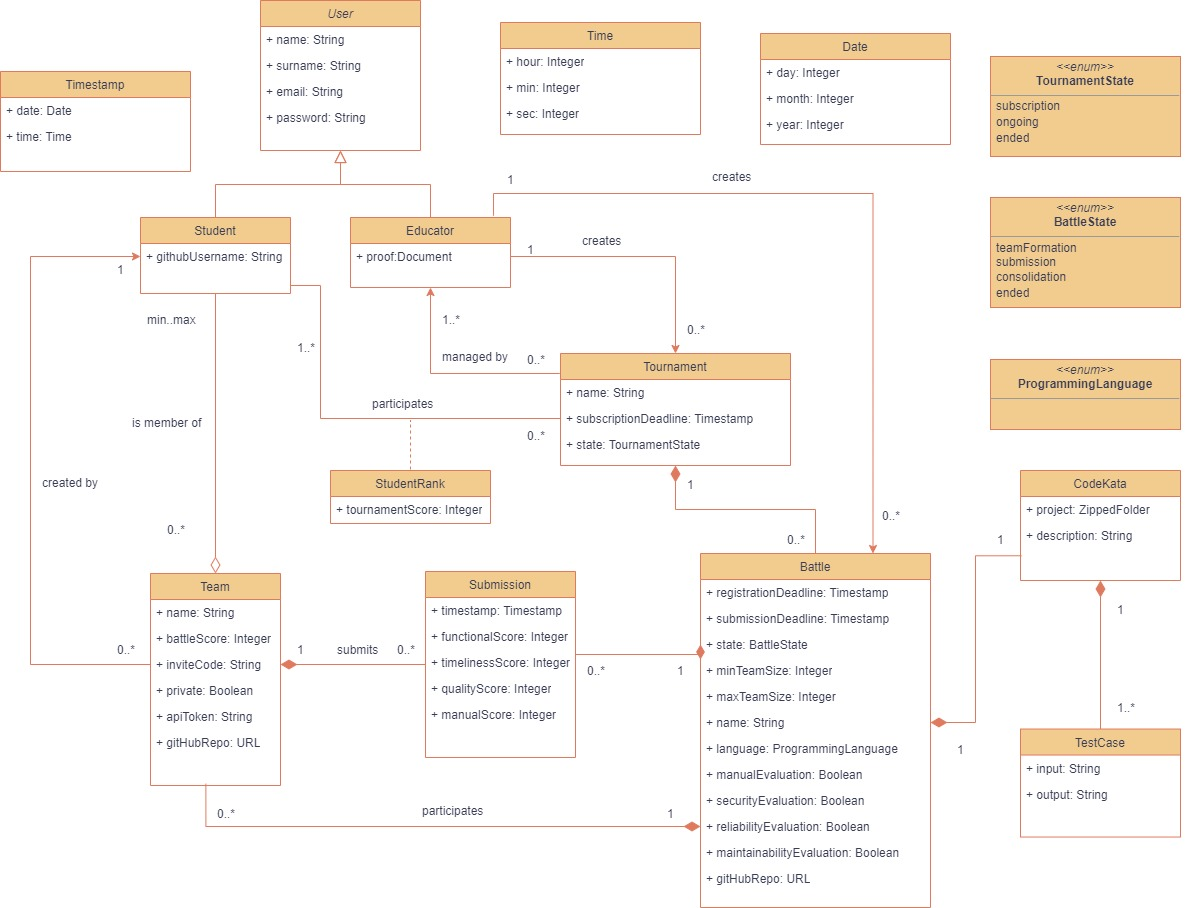
\includegraphics[scale=0.5]{Diagrams/uml_v2.jpg}
    \caption{Domain-level UML diagram}
    \label{class_diagram}
\end{figure}
\newpage
\textbf{ Additional notes on the class diagram:}
\begin{itemize}
    \item the "proofDocument" attribute of the "Educator" class contains a reference to the file through which the educator was verified.
\end{itemize}

\subsubsection{ State diagrams}
In order to provide a complete description of the application domain, here we included the state diagrams relative to tournaments and battles.
\begin{figure}[h]
    \hspace{-20px}
    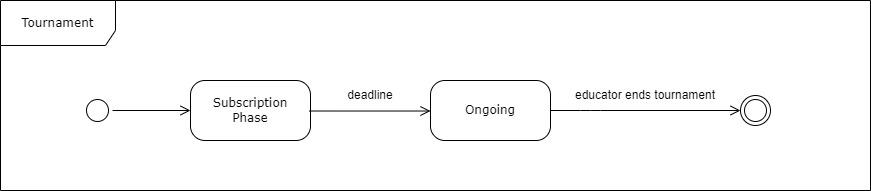
\includegraphics[scale=0.5]{Diagrams/tournament_state.jpg}
    \caption{Tournament state diagram}
    \label{tournament_state}
\end{figure}
\begin{figure}[h]
    \hspace{20px}
    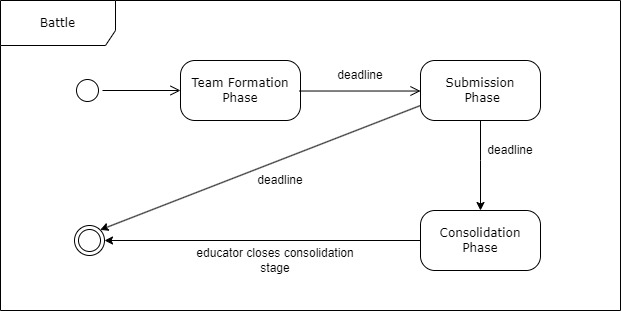
\includegraphics[scale=0.55]{Diagrams/battle_state.jpg}
    \caption{Battle state diagram}
    \label{battle_state}
\end{figure}
\\In particular, in the case of battles, which transition is taken after the submission stage only depends on whether the manual evaluation was enabled or not.

\subsection{Product functions}
\subsubsection{Sign up and Log in}
These functions are used to respectively subscribe to the platform and access the personal area. This will be available to all kind of users, with a little difference between students and educators. Specifically, during the sign up process, the system will start by asking the user if he/she wants to sign up as a student or as an educator.

In the student’s case, the system will ask the new user to enter his/her first and family name, a GitHub username, an email and a password: if the provided email is not already used for another account (of any type) and it really exists a GitHub account associated to the provided username, the system registers the new user. Alternatively, the system allows users to sign up through external identity providers like Google, Facebook and GitHub.

In the educator’s case instead, the system will ask the same information but, instead of the GitHub username (which is not needed in the case of an educator), it will ask him/her a form to explain why is he/she subscribing and a document that proves its identity.

At this point, since notifications will be send via mail in any case, in order to use the system the new user has to verify its email: a verification email is sent to the provided email address containing a link that the user will have to click to confirm it.

Obviously in the future, in order to log in, the user will be asked to provide the email and password entered during the sign up phase: if these match, the system will grant access.
\subsubsection{Manage tournaments}
This functionality is available only to educators and basically represents the main functionality that the platform provides.

In order to initiate a new competition, each educator can decide to create a new tournament. To do this the educator log in to its personal area and then goes to the page listing all the tournaments that he’s ever created (even the ones that have already terminated: the system persists their final ranks and other useful information, see “Create battles” function) or that he has been granted access to. Here the educator can click a button to create a new tournament: a new page is displayed, in which the user has to provide a new (unique) name for the tournament, fix a subscription deadline and, eventually, grant the possibility to other educators to create battles in the context of the new tournament (this is done by fulfilling a search box with their emails such that the system can send them an invitation, which they can accept or not). This is the only setting that can be changed at any time, even while the tournament is active.
\subsubsection{Join a tournament}
This functionality is available only to students. In order to subscribe to a new tournament a student can find inside its personal area a page listing all the tournaments he/she has ever participated to. In this page there’s also a button that allows the student to join a new tournament: a new page is displayed, in which the user has to provide the name (or part of it) of the tournament of interest. The system searches among all the (active) tournaments those whose name is compatible with what the user’s query and returns the list of these.

At this point the student can refine his/her search or select the right tournament from the list and, by doing this, subscribe to it.
\subsubsection{Create a battle}
This functionality is available only to educators. An educator can select an active tournament from the page showing the list of the tournaments he/she has access to: inside the new page that is displayed educators can find data relative to the tournament (e.g. the state of the tournament and how much time before the next) and the students subscribed to it (e.g. actual ranking and list of subscribed students) and also a button that allows them to create a new code kata battle.

By clicking it, the user is brought to a new webpage in which has to provide multiple information:
\begin{itemize}
    \item Battle name
    \item Programming language of use
    \item Upload Code Kata, including project description, automation scripts and test cases
    \item Set minimum and maximum number of students per group
    \item Set registration and final submission deadline
    \item Specify scoring configuration (see “Evaluate a submission” function)
\end{itemize}
At this point the battle is created and the registration phase starts. Once the registration deadline is met, the system will prepare the development environment for each student: specifically, it will create a new public repository on the platform GitHub account and send the relative link to all team leaders, which will need to fork the repository, set up GitHub Actions and invite his/her teammates (if there are) as collaborators.
\subsubsection{Join a battle}
This functionality is available only to students. A student that is subscribed to a tournament is notified upon the creation of a new battle in the context of it. In the case the user is interested into participating, he/she can subscribe to it by creating a team or joining one that has already been created.

As first thing he/she has to access the page relative to the teams for that battle. This can be done in 2 ways:
\begin{itemize}
    \item Directly by clicking the link inside the notification sent through the email.
    \item Go to the page displaying his/her list of tournaments and select the one of the new battle: inside a new page there will be shown the actual rank and the list of battles up to the last,  the active one, which can be selected. If a user selects a battle it has already subscribed to, he/she is brought to the page devoted to its team.
\end{itemize}
Inside a new page it will be displayed the list of available teams and 2 buttons.

The first button allows the student to create a new group: upon click a new page will be shown in which the student has to fill a form to enter all the necessary information. Specifically, the student has to:
\begin{itemize}
    \item Provide a (unique) name for the team
    \item Set the visibility of the group: the creator can toggle a checkbox to specify that the team will be private
\end{itemize}
At this point the system creates 2 random strings that will be univocally associated with the newly created team:
\begin{itemize}
    \item an invite code: this will represent the only way to access private teams and, in general, an alternative way to join teams.
    \item an API token: this will be requested to be included inside the GitHub Actions workflow in order to allow the system to understand which team a solution belongs to.
\end{itemize}  
In this case the student that created the team will be marked as team leader (see “Create battles” functionality). This functionality is particularly important because students that want to participate by their own, need to create a group (in order to be sure, they can set it as private and simply keep the invitation code for theirselves: anyway we must keep in mind that this scenario is available only when the minimum number of students per group is set to 1).

The second button instead allows the student to join an already existing group: this is achieved by allowing the student to search groups by name (in case of private teams, in a following page the student will be asked to provide the right invite code) or by directly providing their invite code: if the specified group does not already contain the maximum number of students for the battle, the system adds the student to the group.
\subsubsection{Submit a solution}
Once the registration phase is over, the submission phase starts: the system provides each student/team a GitHub repository in which the solution code has to be collected (teams of students have to manually guarantee access to all needed collaborators). Then, GitHub Actions has to be set up in each of these repositories in order to enable the necessary workflow: in this way the submission of a new solution is performed by committing and pushing over the repository as we would normally use GitHub for. On push, an API call will notify the platform of the publication of a new solution for that student/team and proceed to evaluate it.
\subsubsection{Evaluate a submission}
The platform provides an automatic evaluation system that is used to score the solutions submitted by the students. Scoring is divided in 2 groups:
\begin{itemize}
    \item \textbf{Automatic evaluation}: this comprises all the aspects that are mandatory to be assessed. These are:
    \begin{itemize}
        \item Correctness, measured in terms of number of test cases solved correctly out of all.
        \item Timeliness, measured in term of time passed between the registration deadline and the last commit.
        \item Quality level: the system uses external tools to evaluate the code with respect to 3 possible aspects that are security, reliability and maintainability (educator decides which to include at battle creation time).
    \end{itemize}
    These aspects are quantified and then combined in a way to return an integer score between 0 and 100.
    \item \textbf{Manual evaluation}: this is an optional evaluation phase that educators can decide to reserve time for (must be indicated at battle creation time). Specifically, in the case the educator has specified it, as soon as the mandatory evaluation has been computed the system allows him/her to manually inspect the code provided by each team: by clicking on the name of the team inside the final rank the system displays a new page in which is shown the link to the team’s GitHub repository and a form that must be filled with an integer score between 0 and 100.\\ The final mark will be computed as the arithmetic average between the automatically assessed score and the one assigned by the educator.
\end{itemize}
\subsubsection{Visualize ranking}
At any time, any user of any kind can visualize the ranking of the tournaments/battles it was involved in by reaching the dedicated page inside their personal area and selecting the tournament/battle of interest. Battle ranks are computed considering the highest score of each team, while the tournament ranks are computed considering, for each student, the sum of the scores assigned to its teams during battles in the context of that tournament.
\subsubsection{Send notification}
The system sends notifications (by means of emails) to its users in the following cases:
\begin{itemize}
    \item on tournament creation, all the students subscribed to the platform are notified
    \item on battle creation, all the students subscribed to the tournament the new battle will belong to are notified
    \item as soon as the final battle score is available, all the students belonging to the same team are notified
    \item on tournament closure, all subscribed students are notified
\end{itemize}

\subsection{User characteristics}
As we’ve already said many times, the system is meant to be used by 2 kind of users:
\begin{itemize}
    \item \textbf{Educators}: this is the type of users that uses the platform to create competitions. They can create tournaments and battles and, eventually, evaluate the solutions provided by students. They must have a good knowledge of how to create valid automation scripts and have a basic understanding of how to use a web browser.
    \item \textbf{Students}: these are the users that will use the platform to be evaluated or simply to take part in a competition. They can subscribe to tournaments and battles, join groups of students and submit solutions. They are required to have a good knowledge of how to properly setup a GitHub repository and of all the programming languages involved in the battles.
\end{itemize} 

\subsection{Assumptions, dependencies and constraints}
\subsubsection{Domain assumptions}
\begin{enumerate}[label=$\bullet$ \textbf{D\arabic*:}]
    \item Users have access to a stable and reliable internet connection to interact with the CKB platform.
    \item Supported programming languages are limited to popular options like Java, Python and C++.
    \item Registered educators are all legitimate and verified.
    \item Educators upload correct test cases and well-structured Code Kata projects.
    \item Students are expected to engage in Code Kata Battles with integrity, without resorting to plagiarism or cheating (e.g. inviting more or different collaborators with respect to the ones inside the team).
    \item Maximum number of students per group an educator can set will always be bounded (e.g. less than 4).
    \item Every student has a GitHub account.
    \item Students will fork the Code Kata GitHub repository once ready.
    \item Students know how to setup a GitHub Actions worfkflow.
    \item Only one student per group will perform the steps needed to set-up the team's repository and the GitHub Actions workflow.
    \item Static analysis tools are able to quantify the specified code quality aspects.
    \item Students use external communication channels.
\end{enumerate}

%------------------------------------------------------------------------------------------------------------------------------------------------
\clearpage
{\color{Blue}{\section{Specific Requirements}}}
\label{sect:requirements}
\subsection{External Interface Requirements}
\subsubsection{User Interfaces}
The platform will have a web interface accessible via browser from both students and educators. 
Now, some mockups of the main pages of the platform will be presented, organized by functionality.

\begin{enumerate}[label=\textbf{F\arabic*)}]
    \item \textbf{Signup and Login}\\
    \begin{figure}[H]
        \centering
        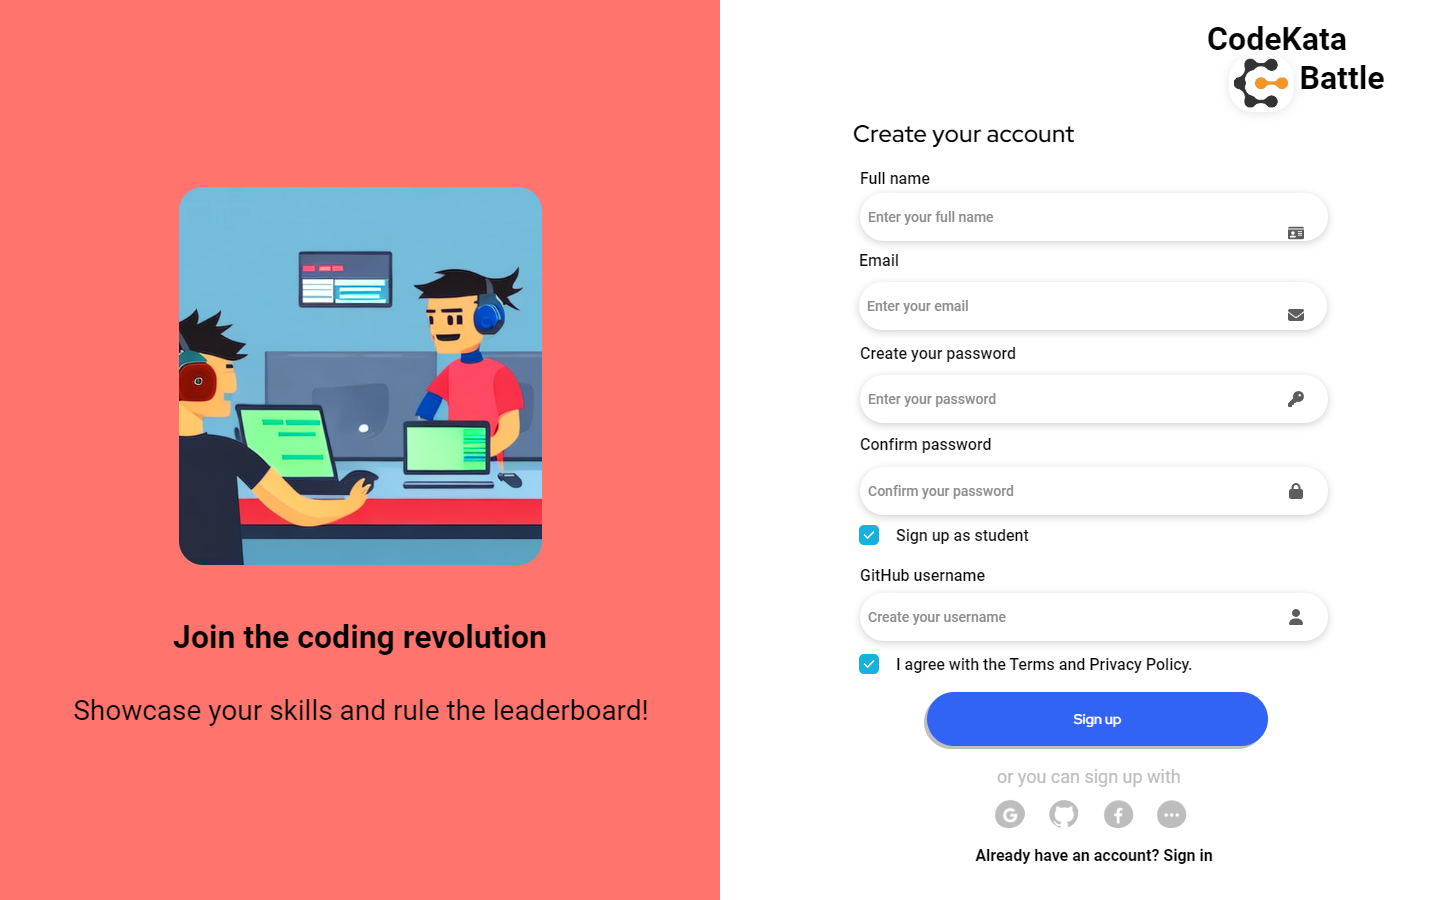
\includegraphics[width=0.8\textwidth]{Mockups/1_signup.png}
        \caption{Signup page}
    \end{figure}
    \begin{figure}[H]
        \centering
        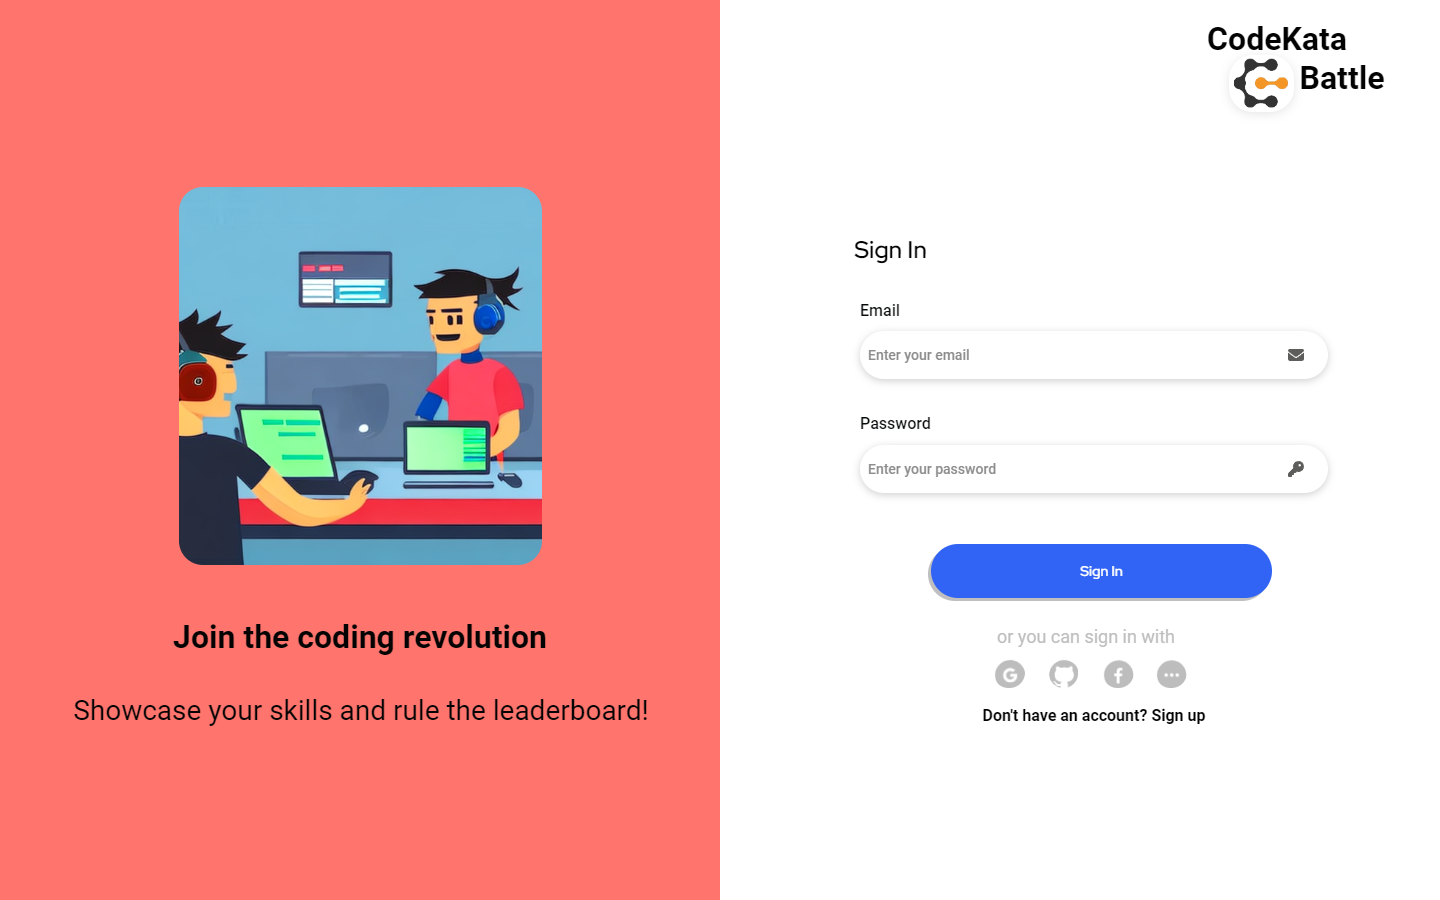
\includegraphics[width=0.8\textwidth]{Mockups/2_login.png}
        \caption{Login page}
    \end{figure}

    \item \textbf{Home page}\\
    \begin{figure}[H]
        \centering
        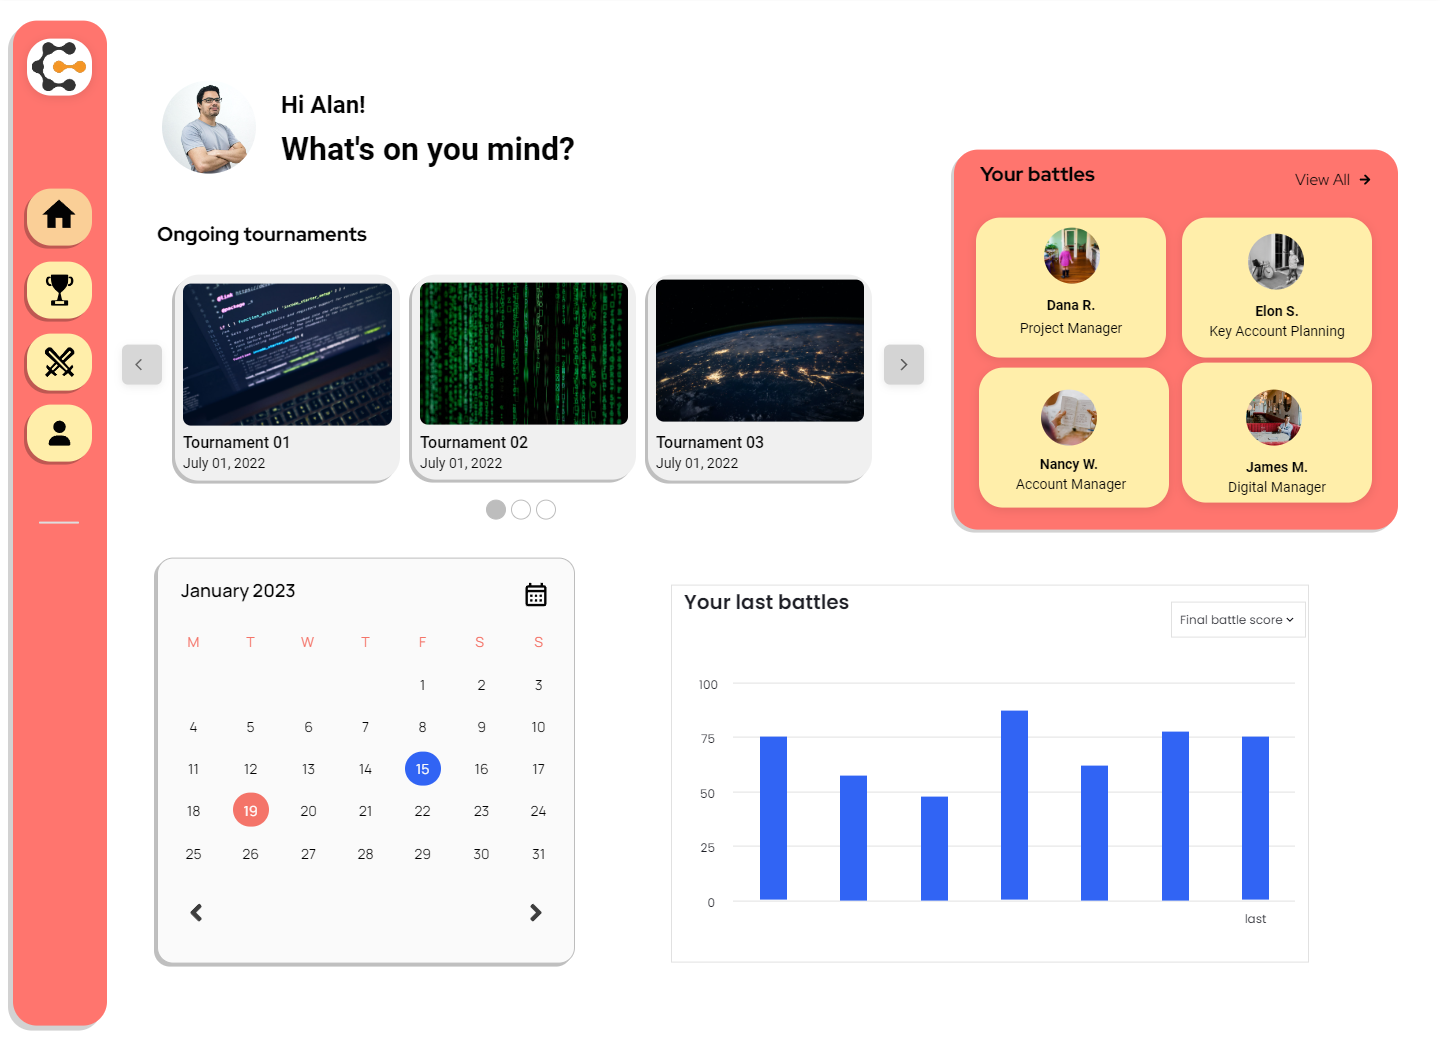
\includegraphics[width=0.8\textwidth]{Mockups/3_student_homepage.png}
        \caption{Home page from the perspective of an user logged as "Student"}
    \end{figure}

    \item \textbf{Tournaments}\\
    \begin{figure}[H]
        \centering
        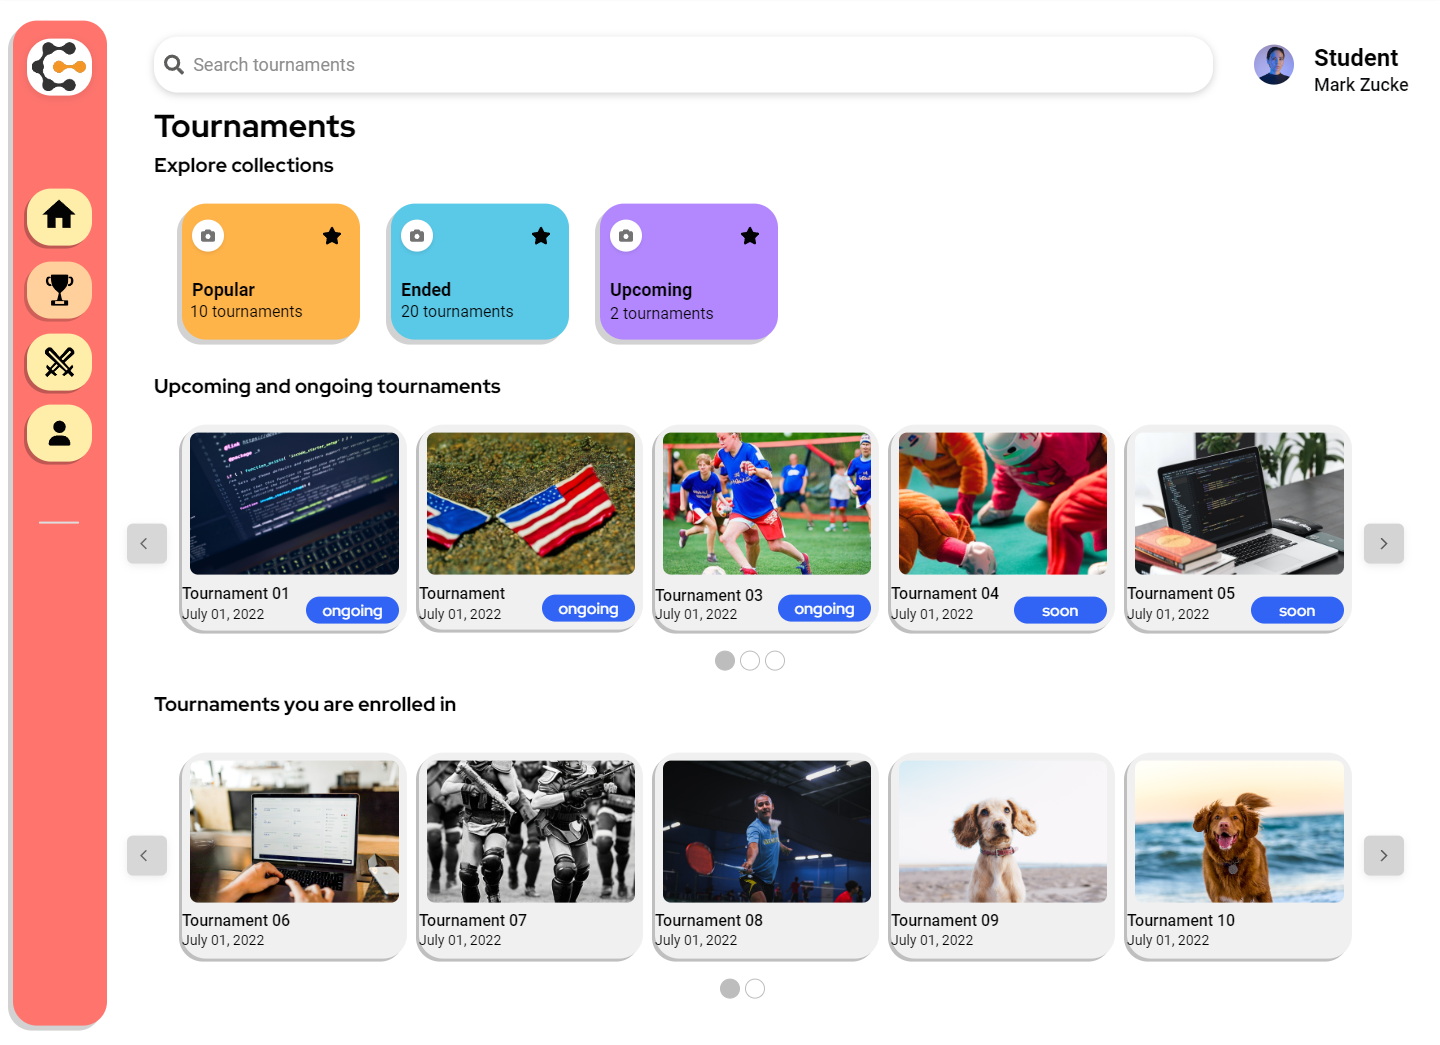
\includegraphics[width=0.8\textwidth]{Mockups/4_student_tournaments.png}
        \caption{Tournaments page from the perspective of an user logged as "Student"}
    \end{figure}
    \begin{figure}[H]
        \centering
        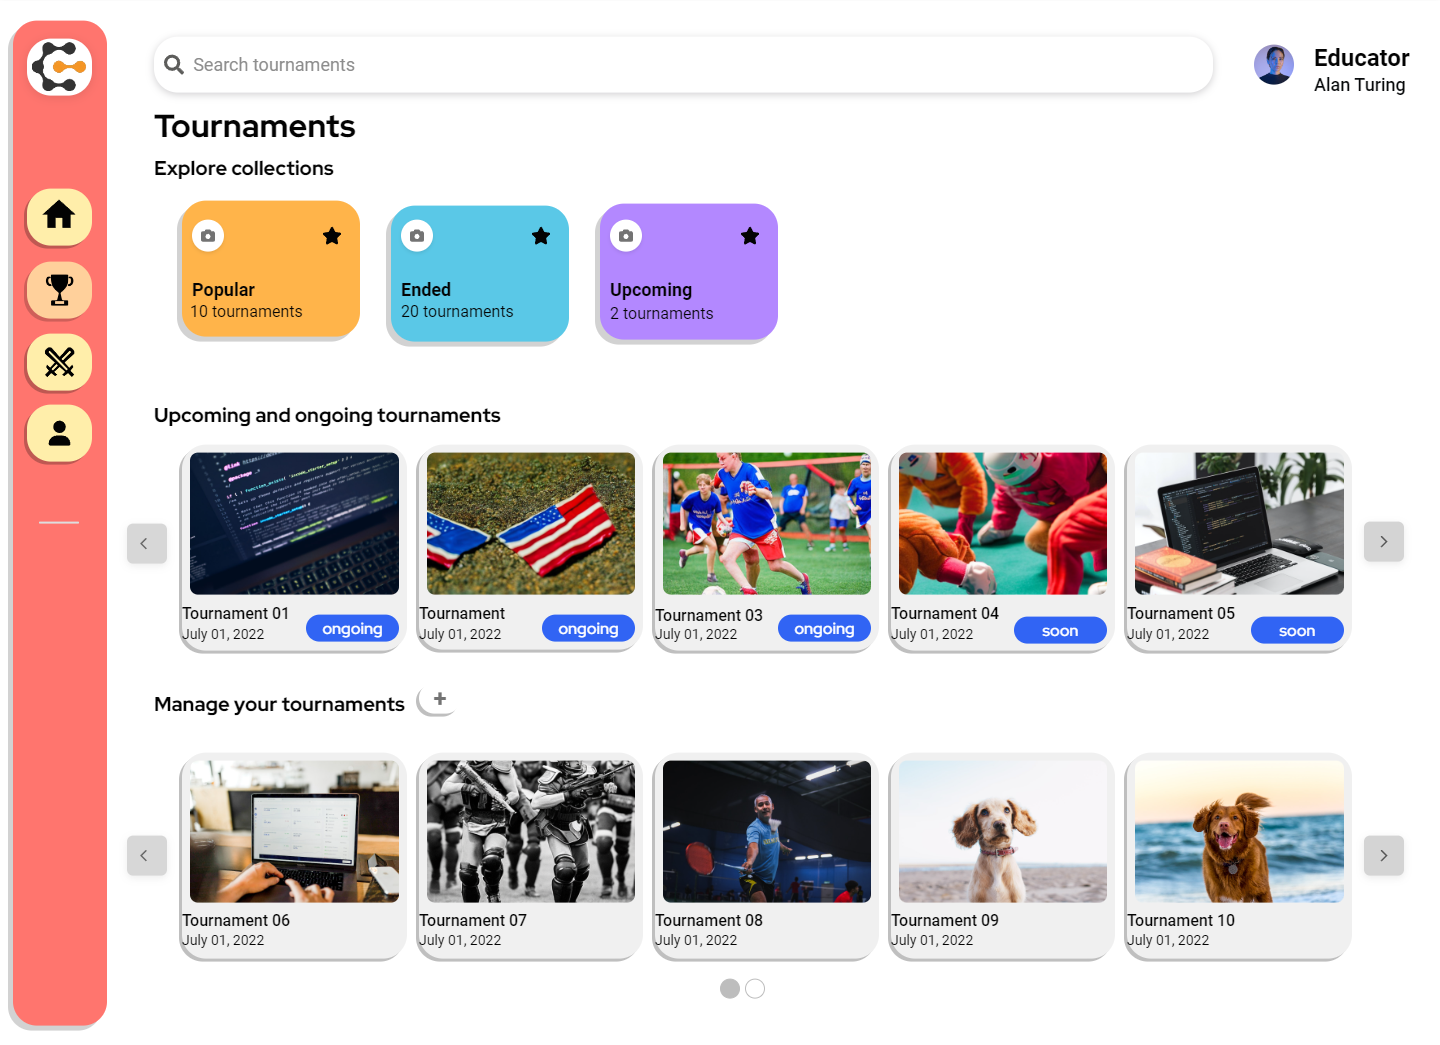
\includegraphics[width=0.8\textwidth]{Mockups/5_educator_tournaments.png}
        \caption{Tournaments page from the perspective of an user logged as "Educator"}
    \end{figure}
    \begin{figure}[H]
        \centering
        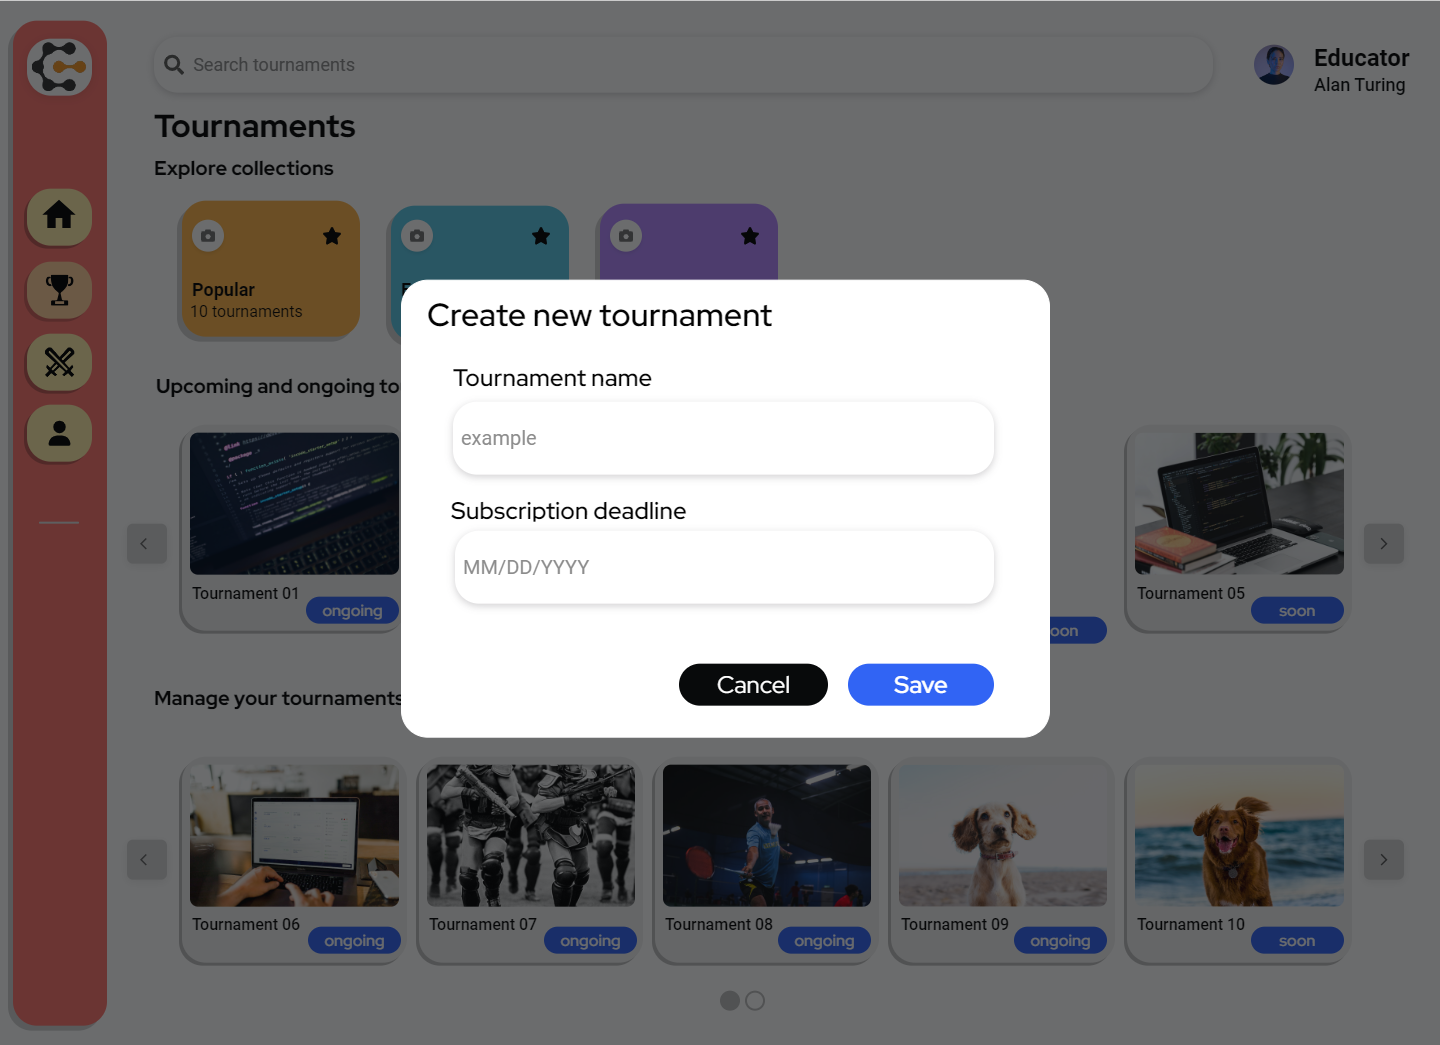
\includegraphics[width=0.8\textwidth]{Mockups/6_educator_create_tournament.png}
        \caption{Page used from Educators to create a new tournament}
    \end{figure}
    \begin{figure}[H]
        \centering
        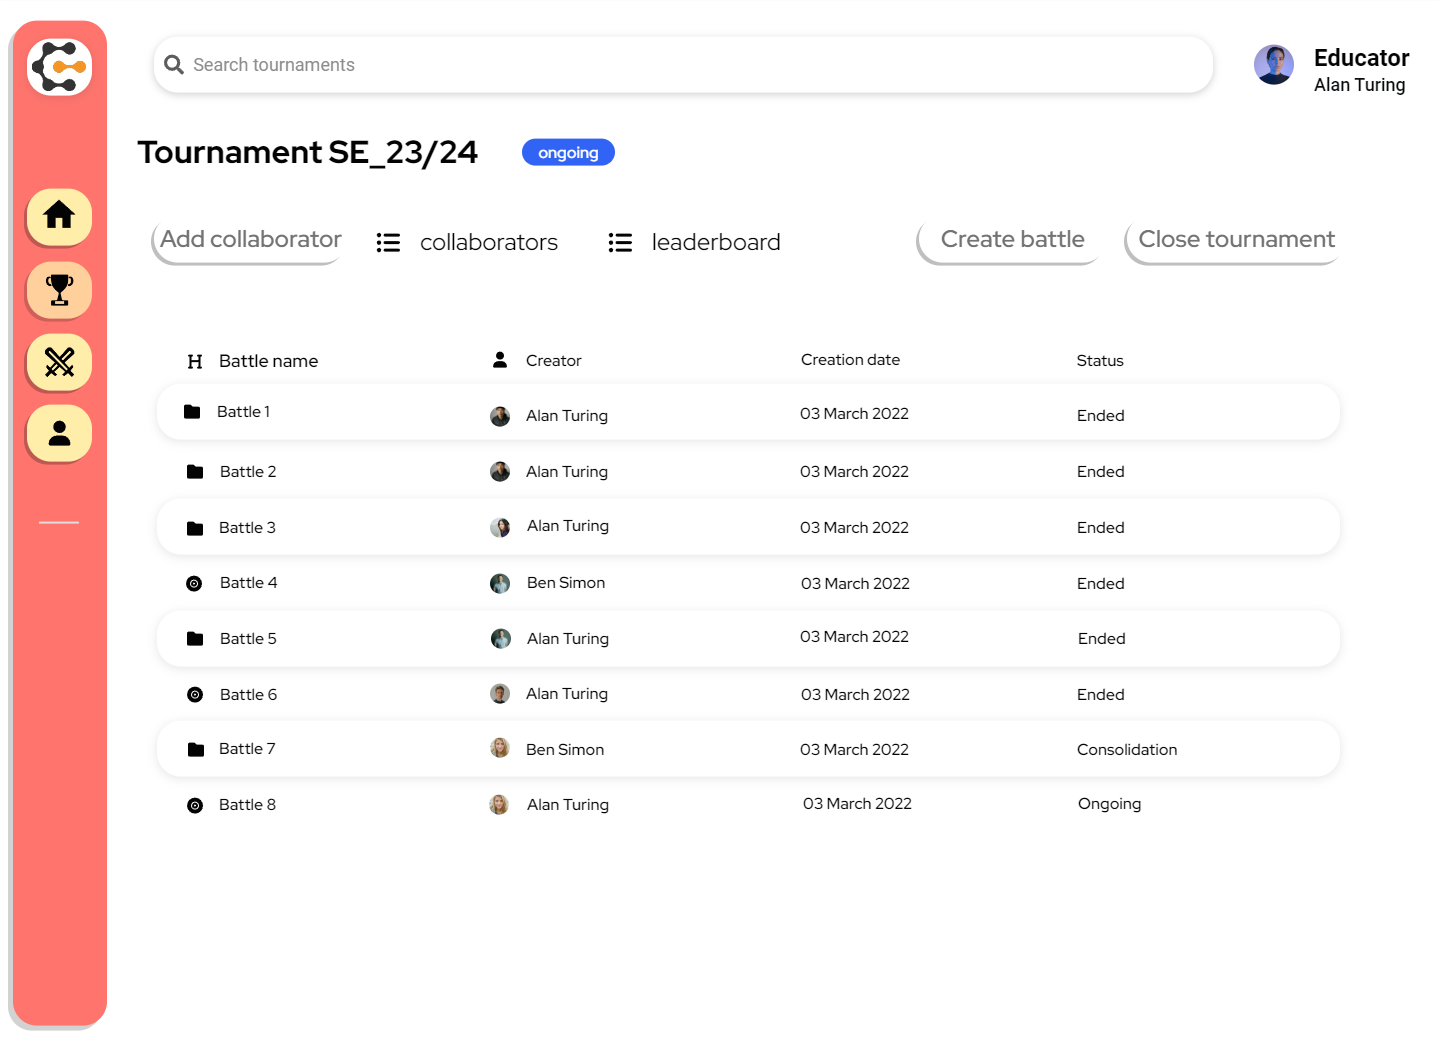
\includegraphics[width=0.8\textwidth]{Mockups/7_educator_manages_tournament.png}
        \caption{Page used from Educators to manage the main settings of a tournament}
    \end{figure}
    \begin{figure}[H]
        \centering
        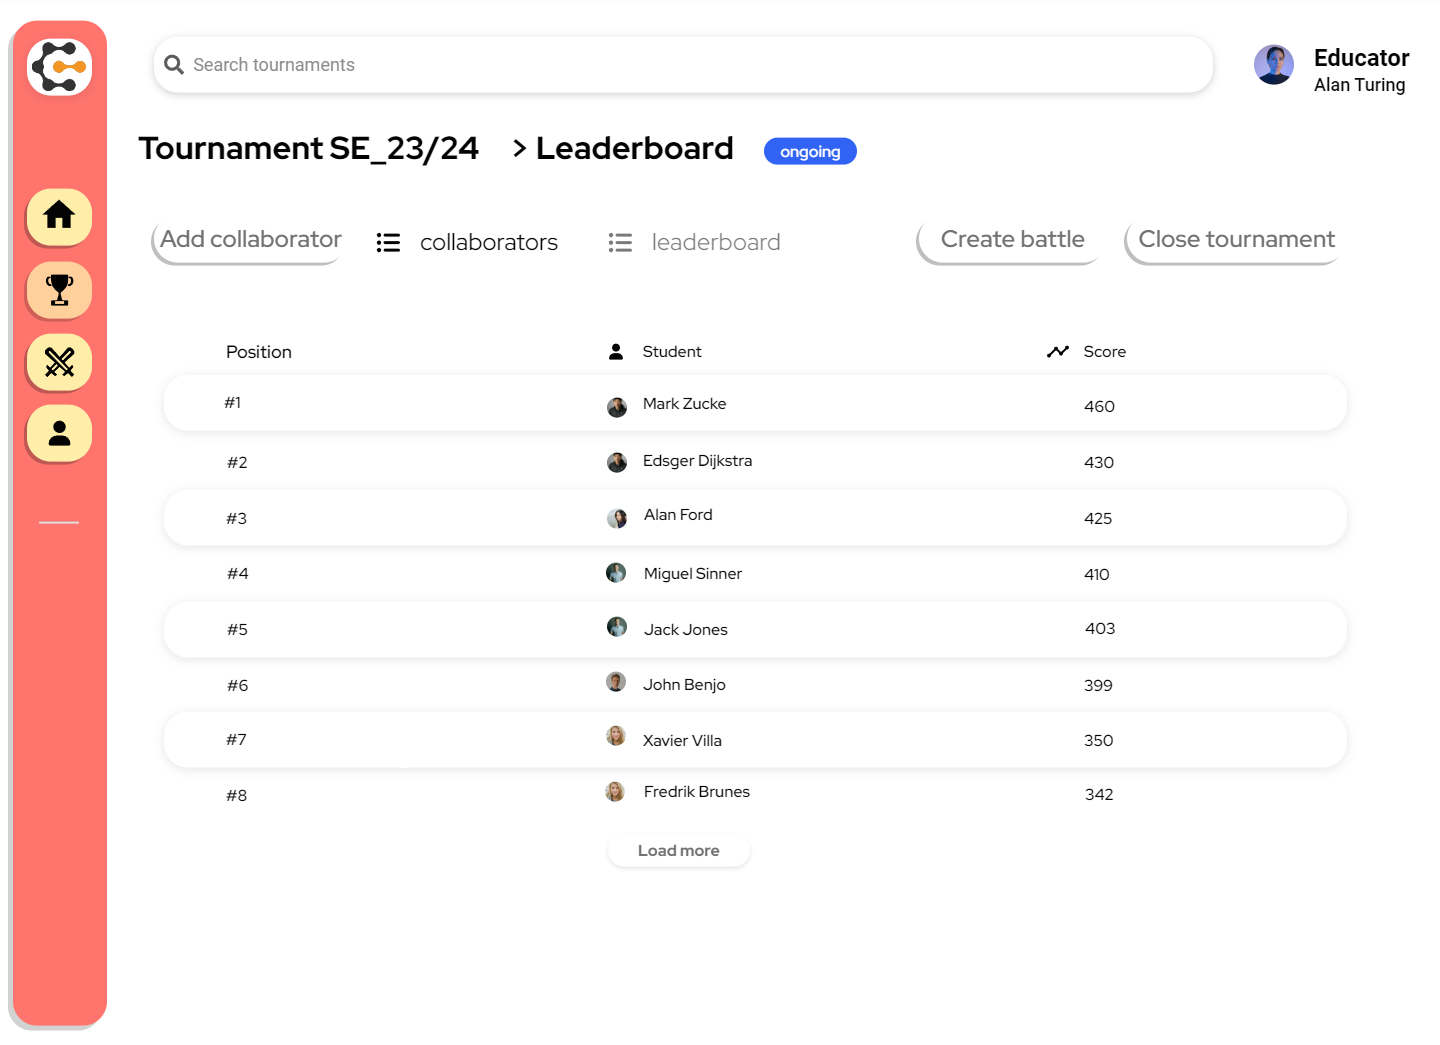
\includegraphics[width=0.8\textwidth]{Mockups/8_educator_tournament_leaderboard.png}
        \caption{Page used from Educators to see the leaderboard of a tournament}
    \end{figure}
    \begin{figure}[H]
        \centering
        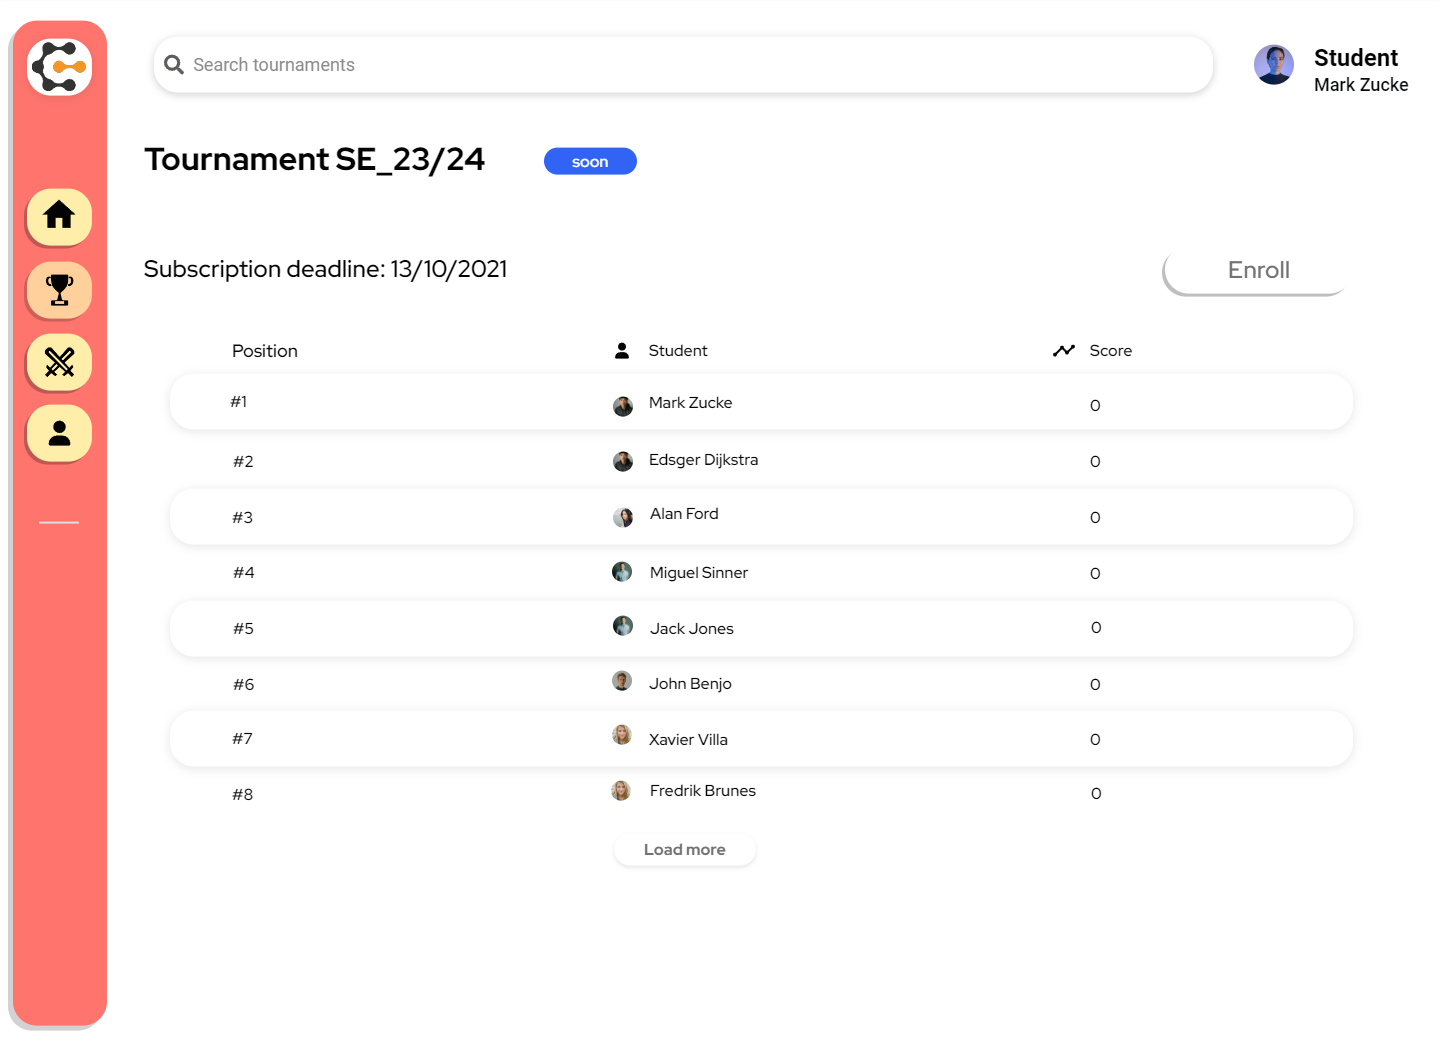
\includegraphics[width=0.8\textwidth]{Mockups/9_student_tournament_subscription.png}
        \caption{Page used from Students to subscribe to a tournament}
    \end{figure}

    \item \textbf{Battles}\\
    \begin{figure}[H]
        \centering
        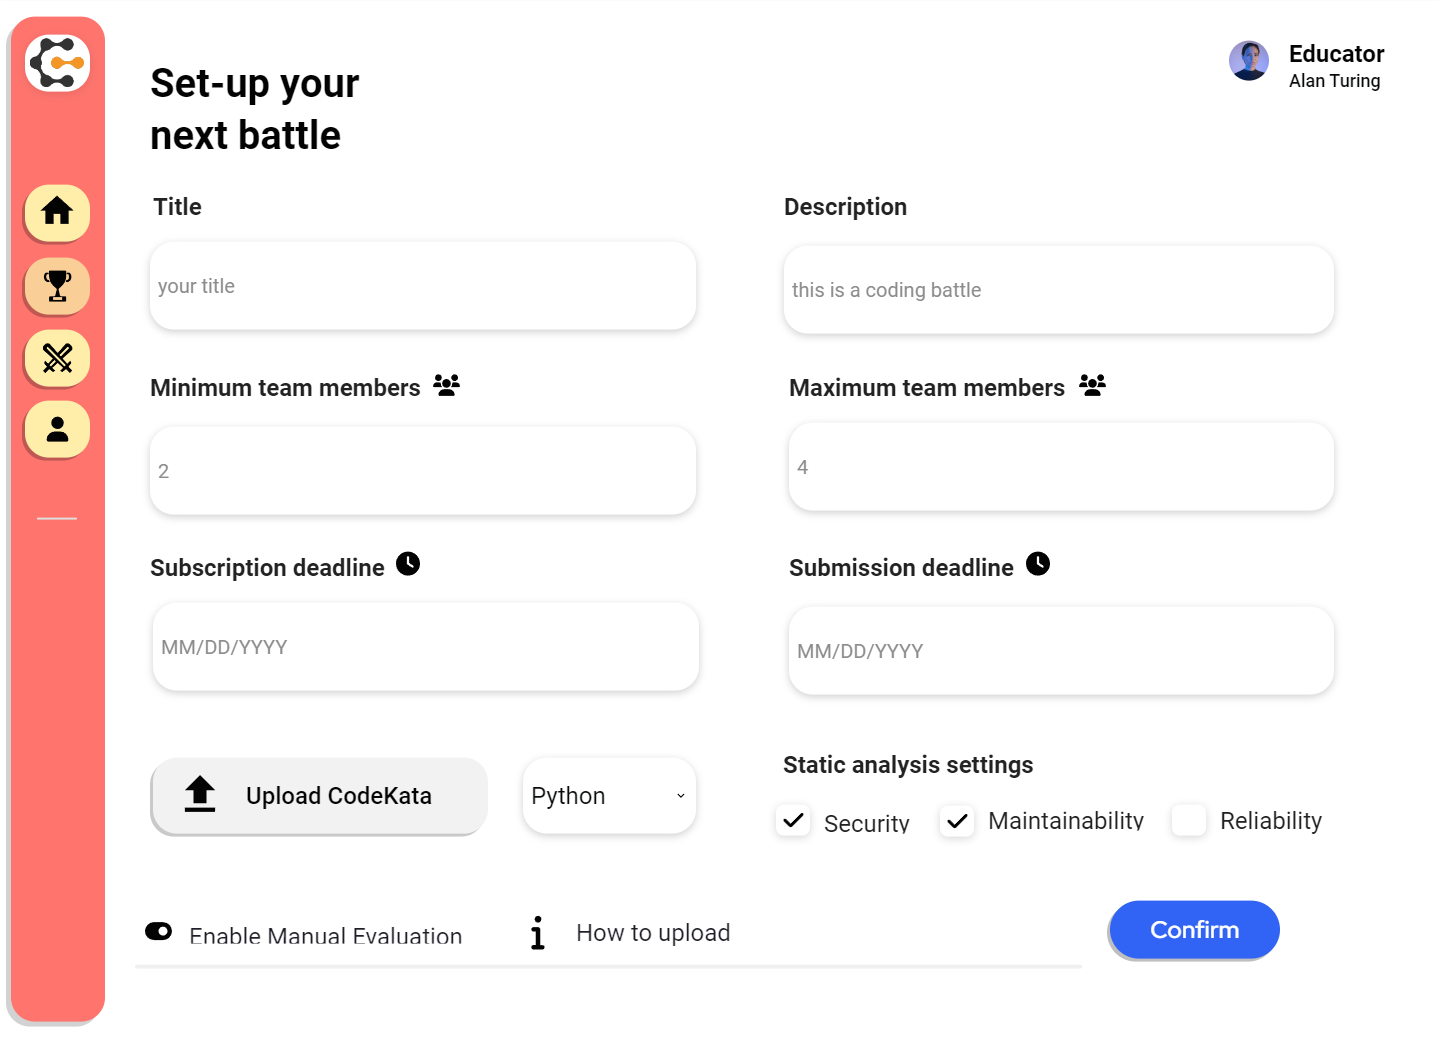
\includegraphics[width=0.8\textwidth]{Mockups/10_educator_create_battle.png}
        \caption{Page used from Educators to create a new battle}
    \end{figure}
    
    \item \textbf{Teams}\\
    \begin{figure}[H]
        \centering
        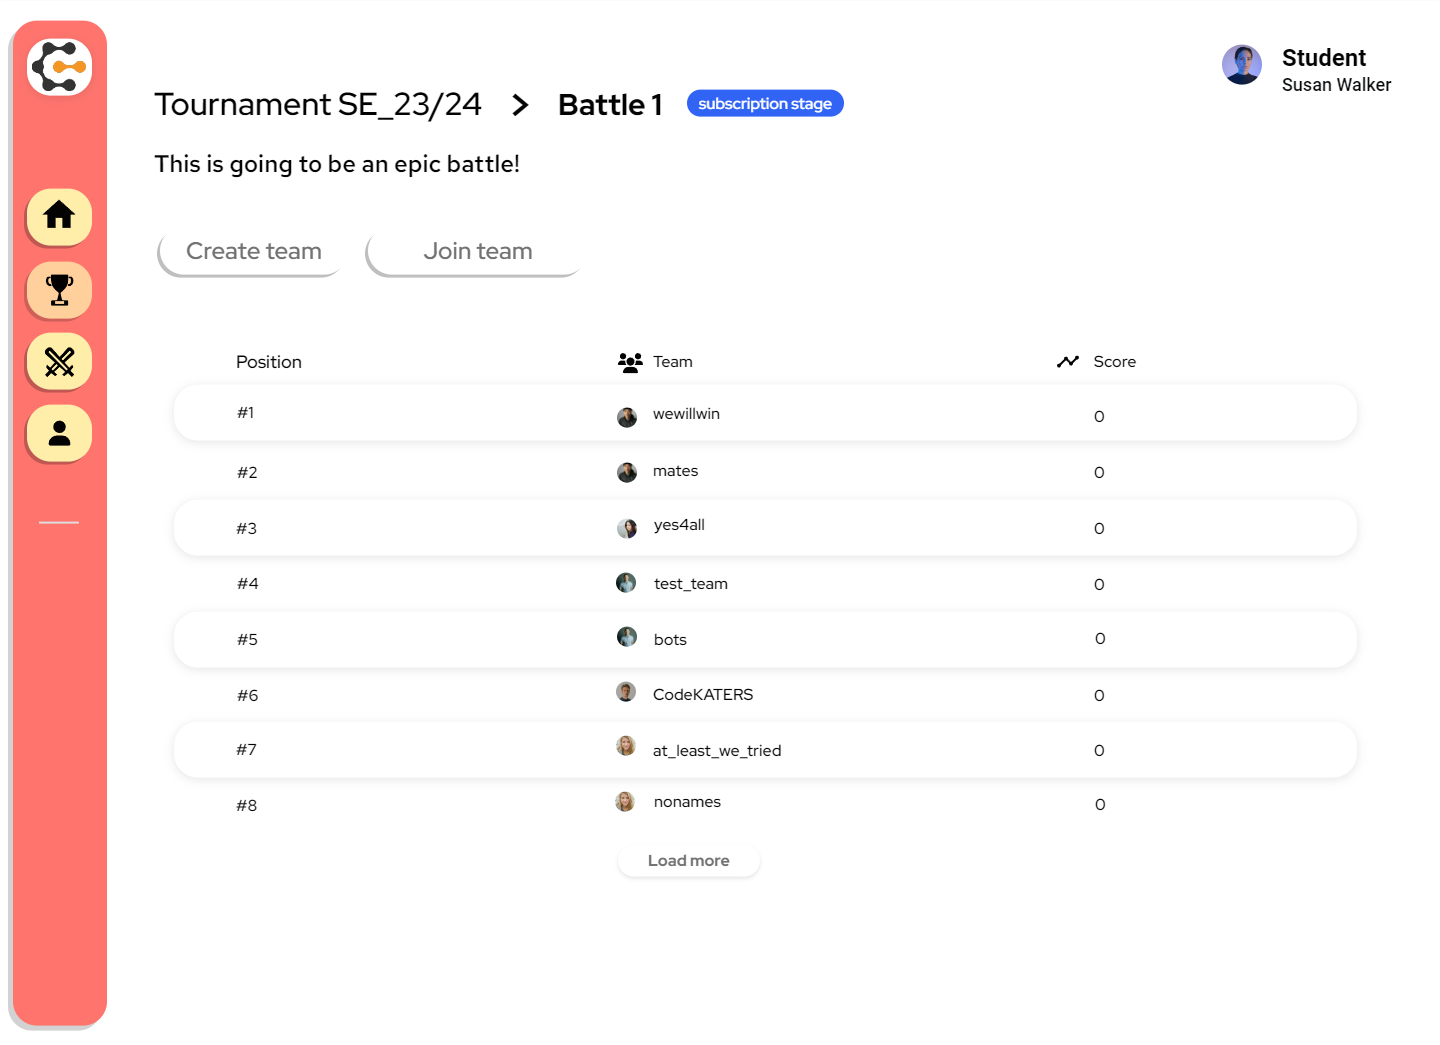
\includegraphics[width=0.8\textwidth]{Mockups/11_student_battle_subscription.png}
        \caption{Page used from Students to subscribe to a battle}
    \end{figure}
    \begin{figure}[H]
        \centering
        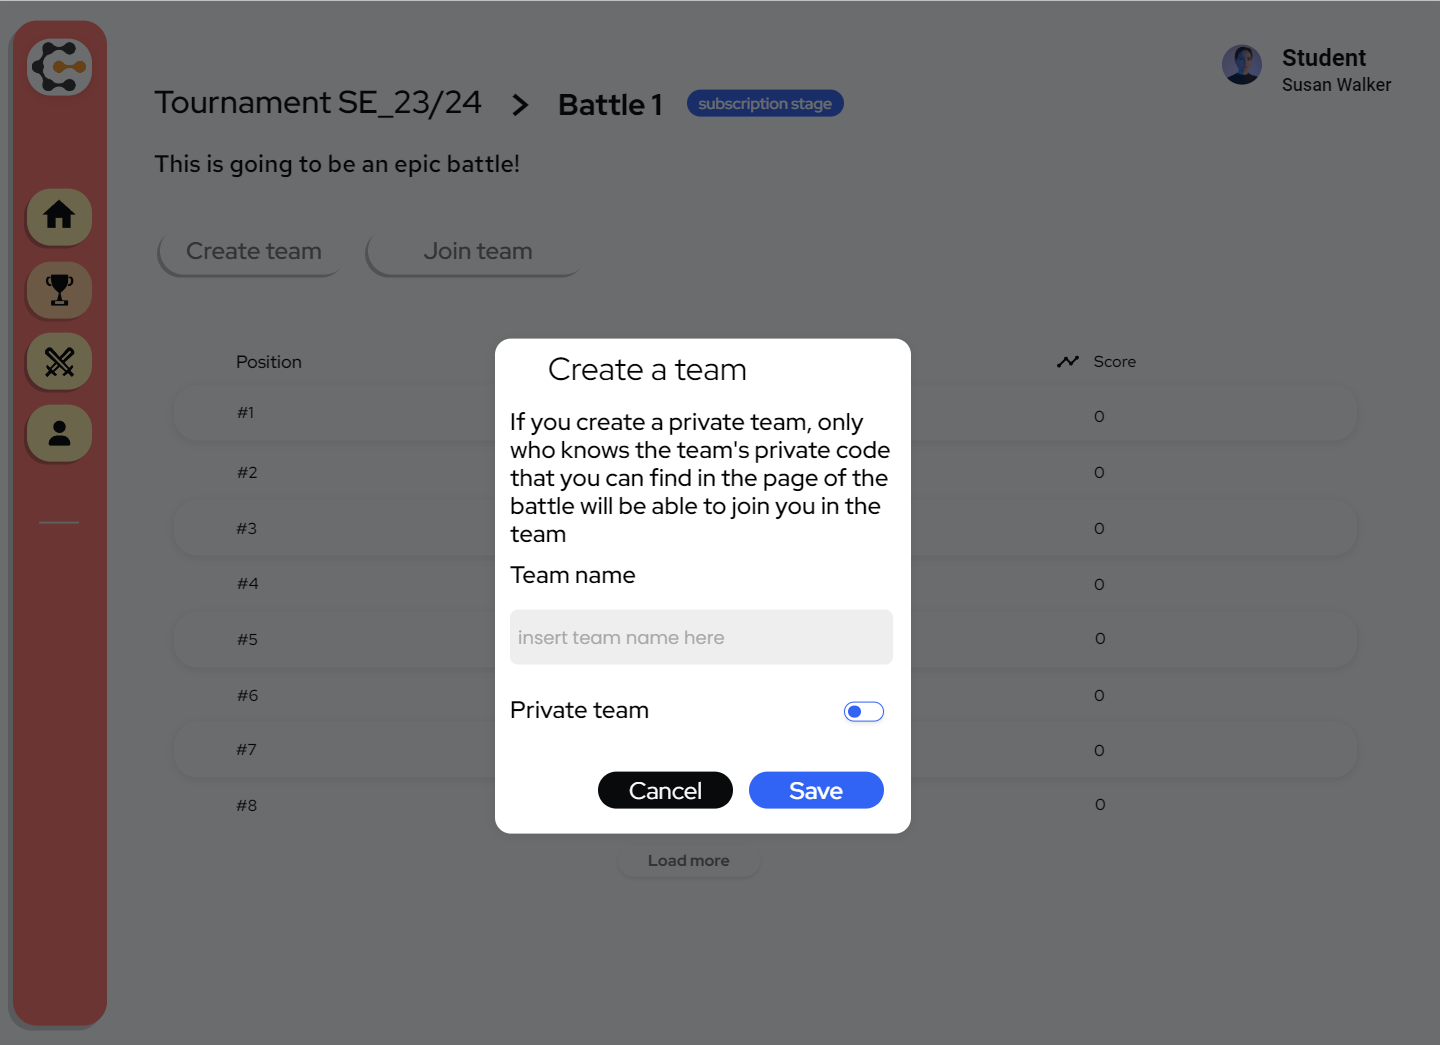
\includegraphics[width=0.8\textwidth]{Mockups/12_student_create_team.png}
        \caption{Page used from Students to create a new team}
    \end{figure}
    \begin{figure}[H]
        \centering
        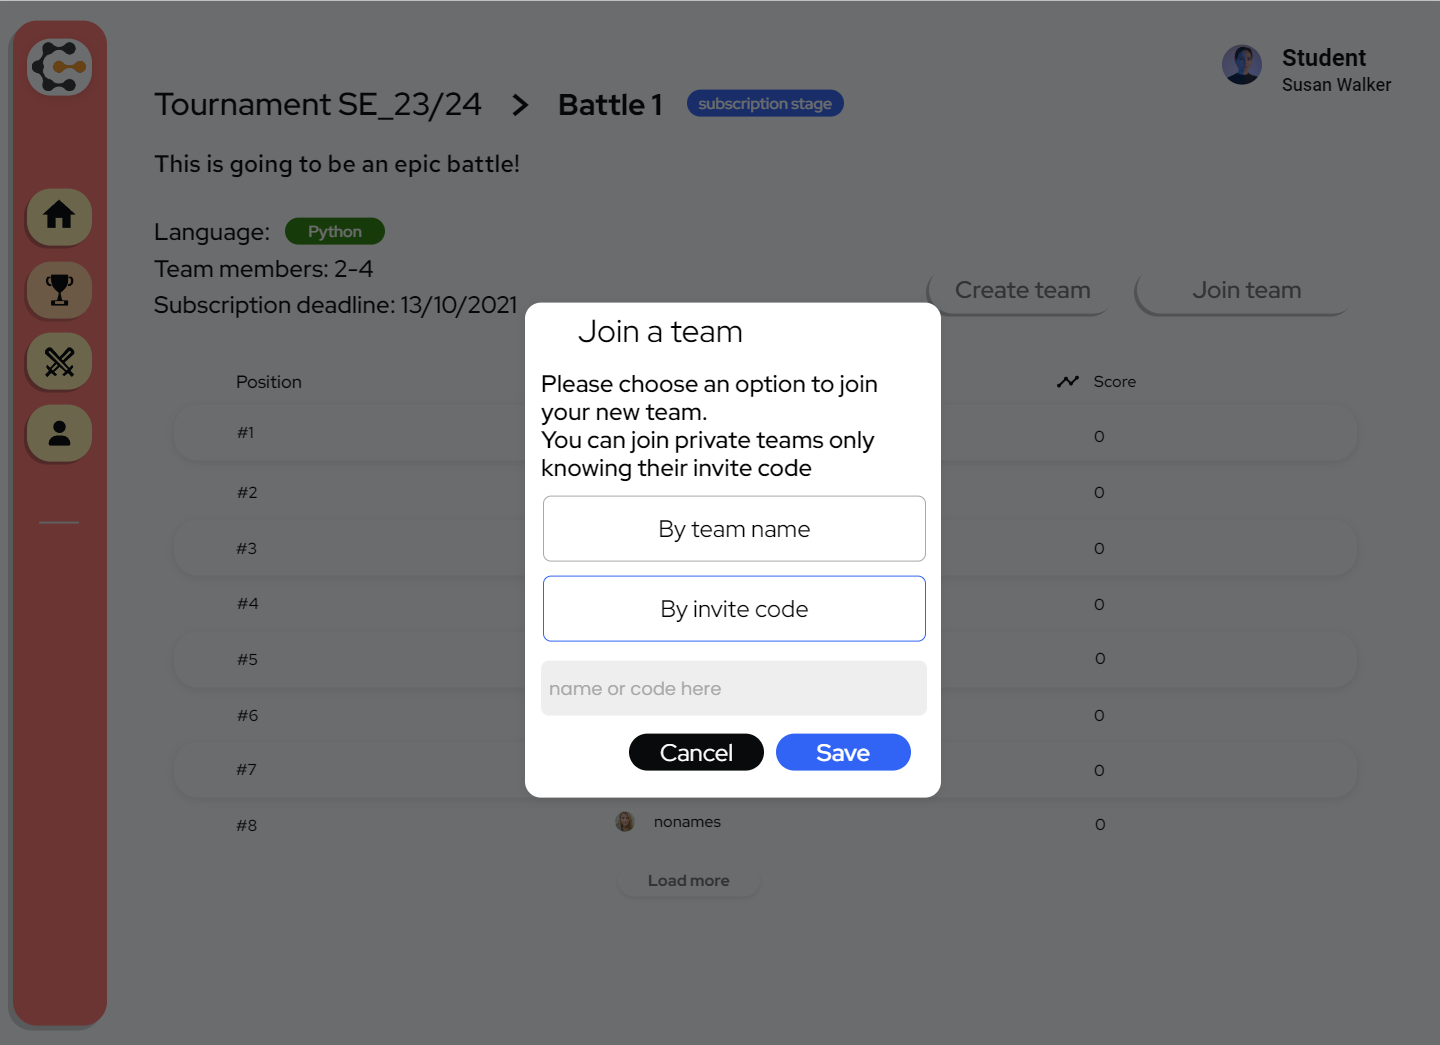
\includegraphics[width=0.8\textwidth]{Mockups/13_student_join_team.png}
        \caption{Page used from Students to join a team}
    \end{figure}
    \begin{figure}[H]
        \centering
        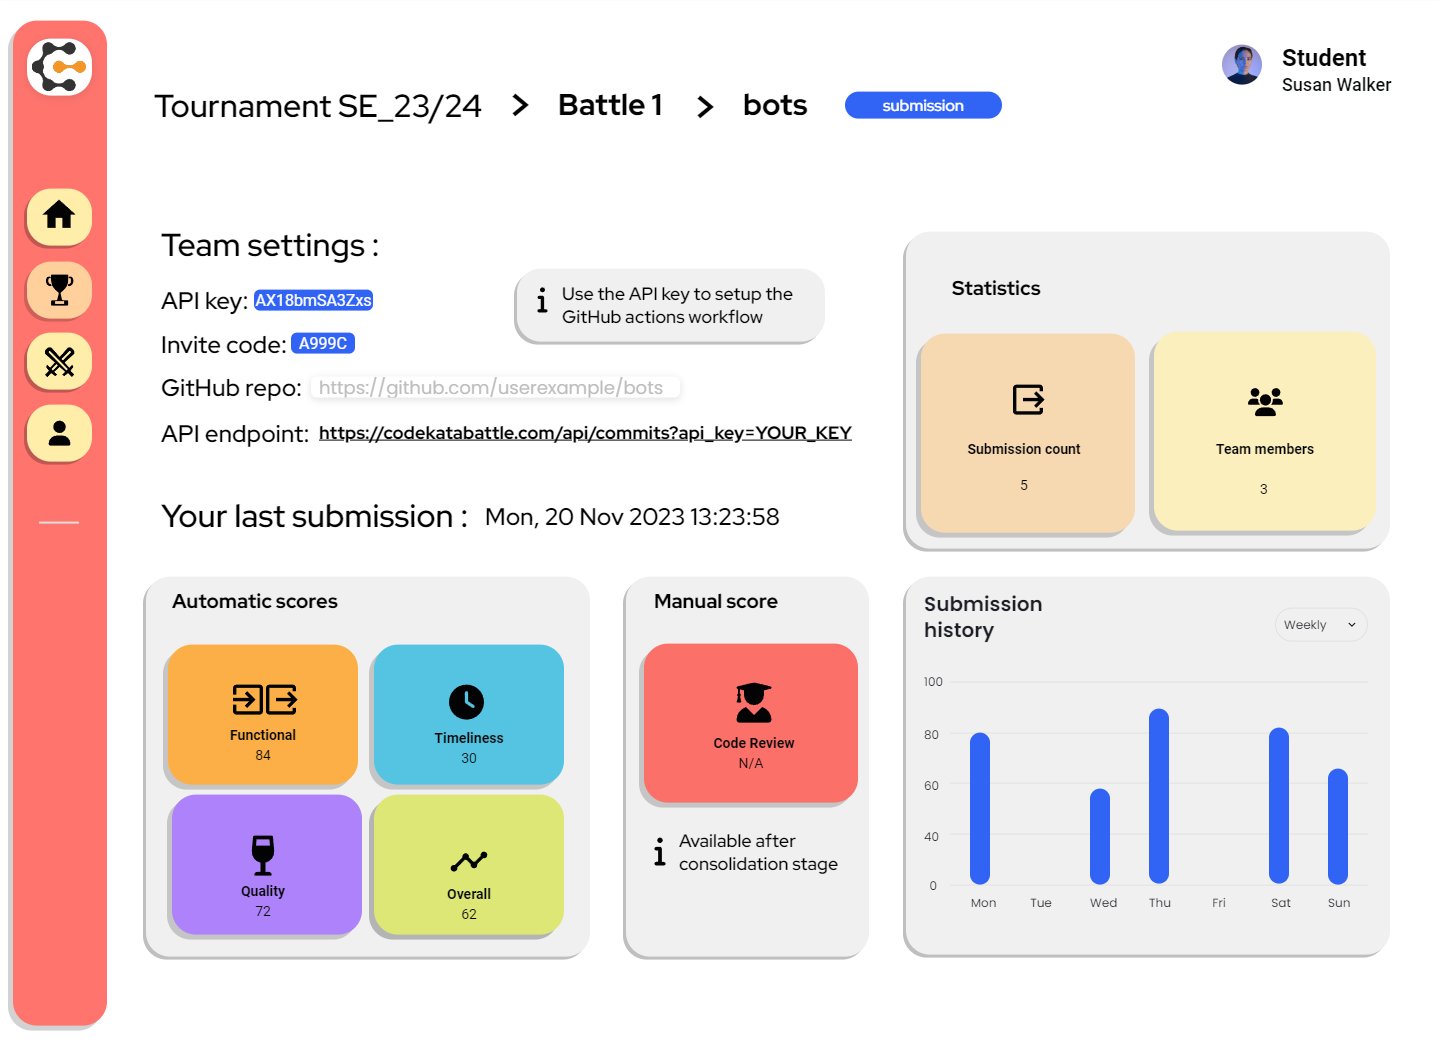
\includegraphics[width=0.8\textwidth]{Mockups/15_student_team.png}
        \caption{Page used from Students to manage the settings of their team}
    \end{figure}
    
    \item \textbf{Evaluation}\\
    \begin{figure}[H]
        \centering
        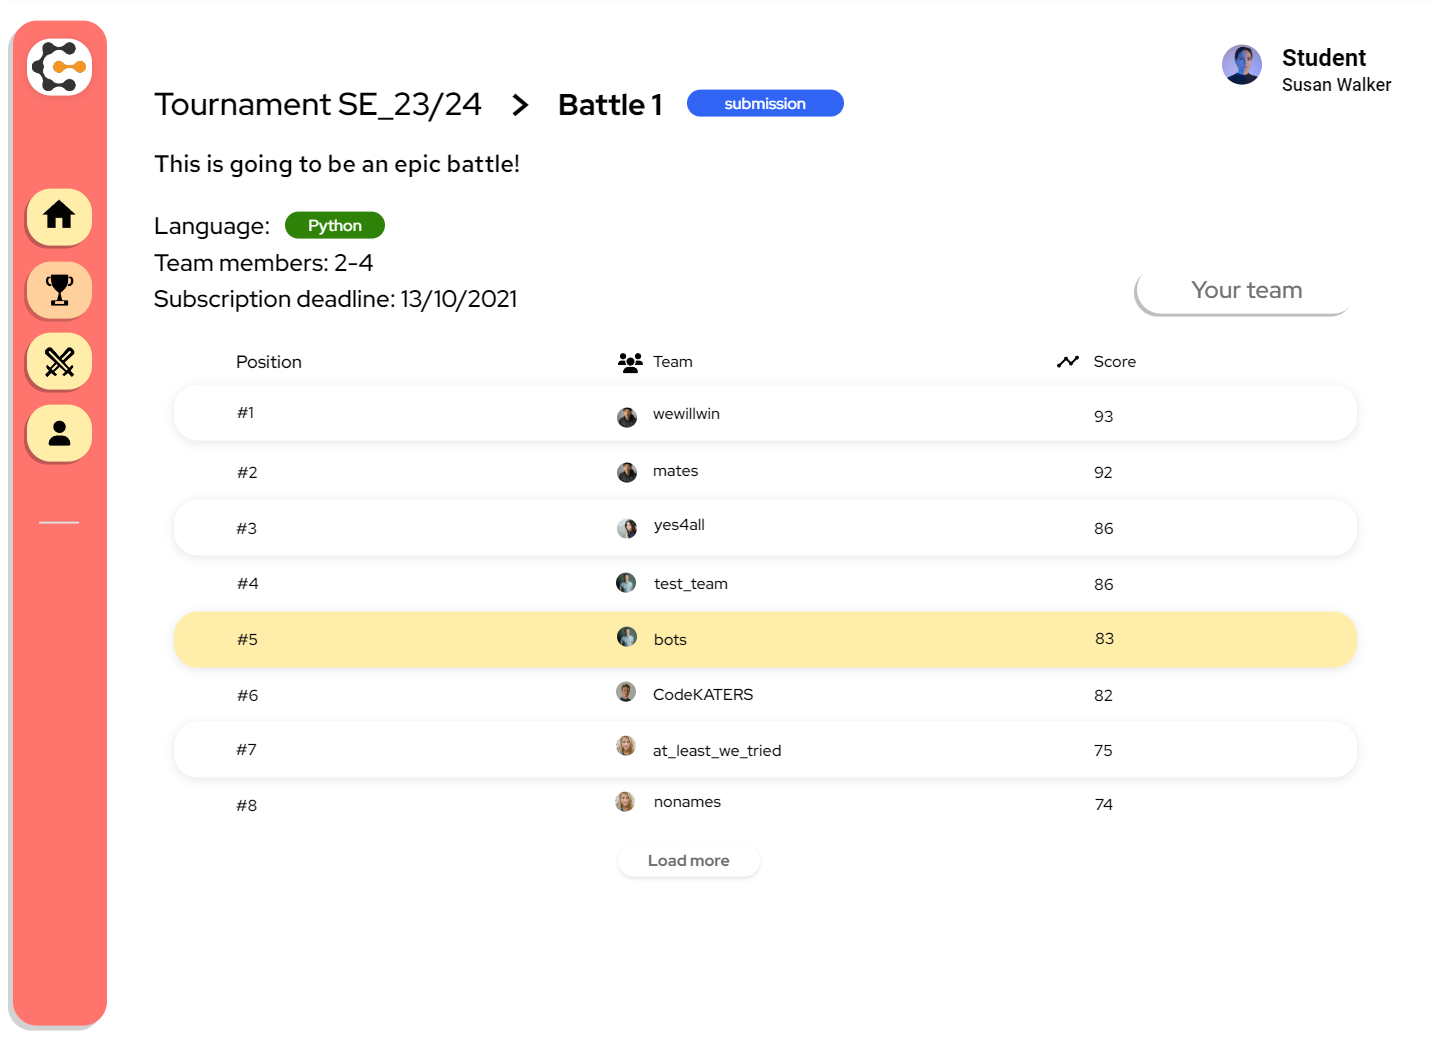
\includegraphics[width=0.8\textwidth]{Mockups/14_student_battle_submission.png}
        \caption{Page used from Students once they have submitted a new solution for a battle}
    \end{figure}
    \begin{figure}[H]
        \centering
        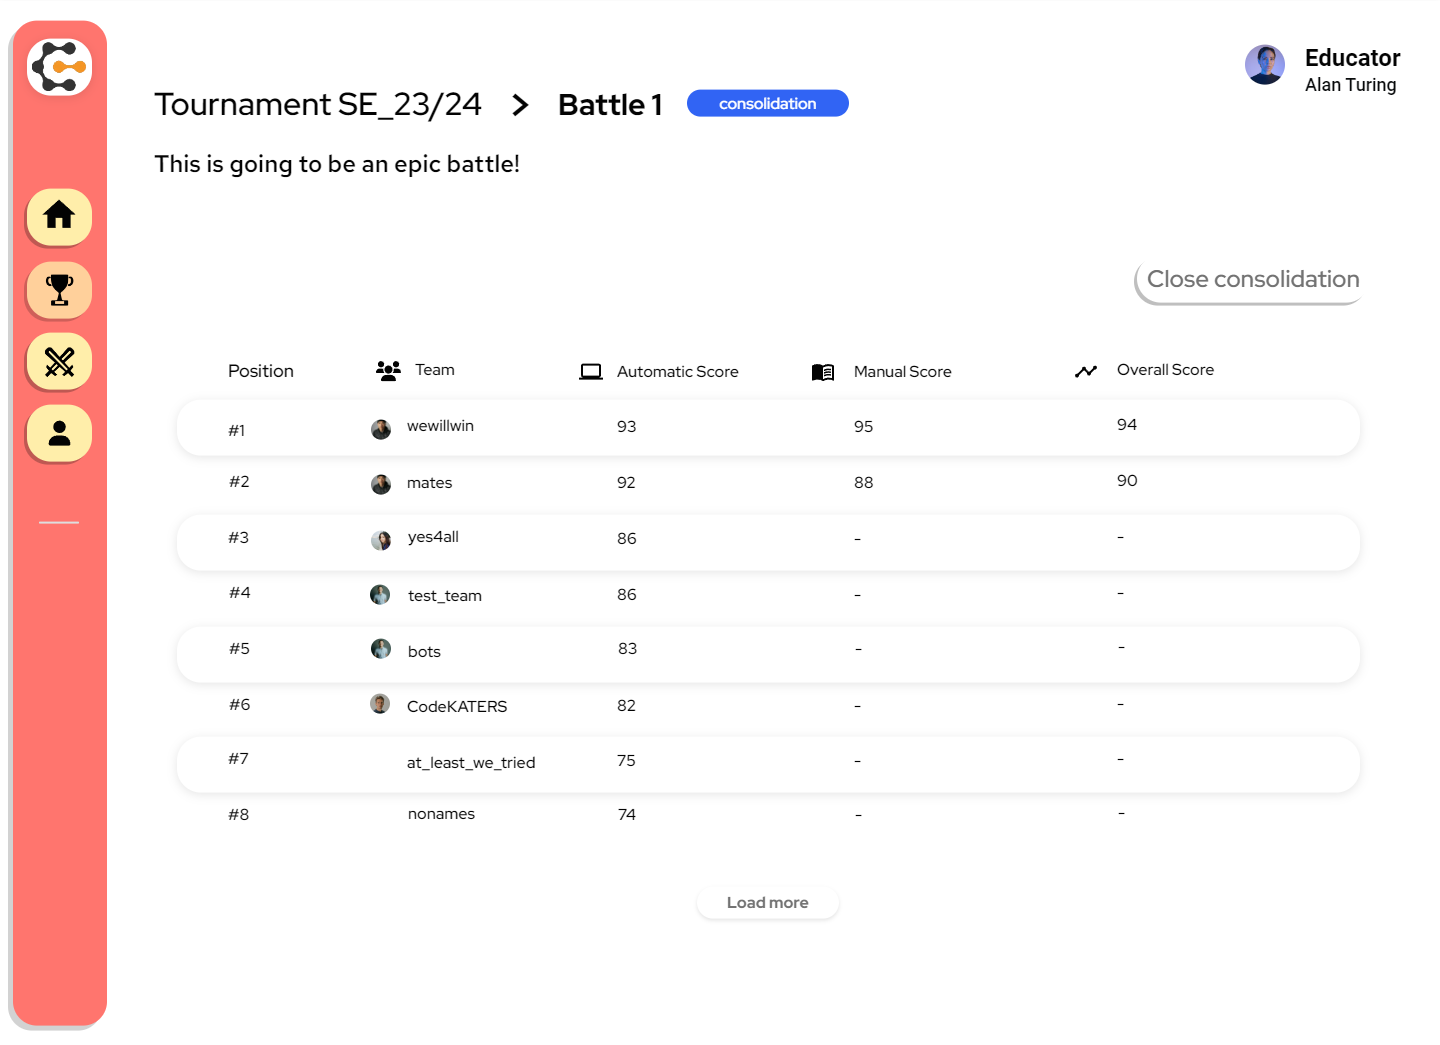
\includegraphics[width=0.8\textwidth]{Mockups/16_educator_battle_consolidation.png}
        \caption{Page used from Educators to manage the Consolidation Stage of a battle}
    \end{figure}
    \begin{figure}[H]
        \centering
        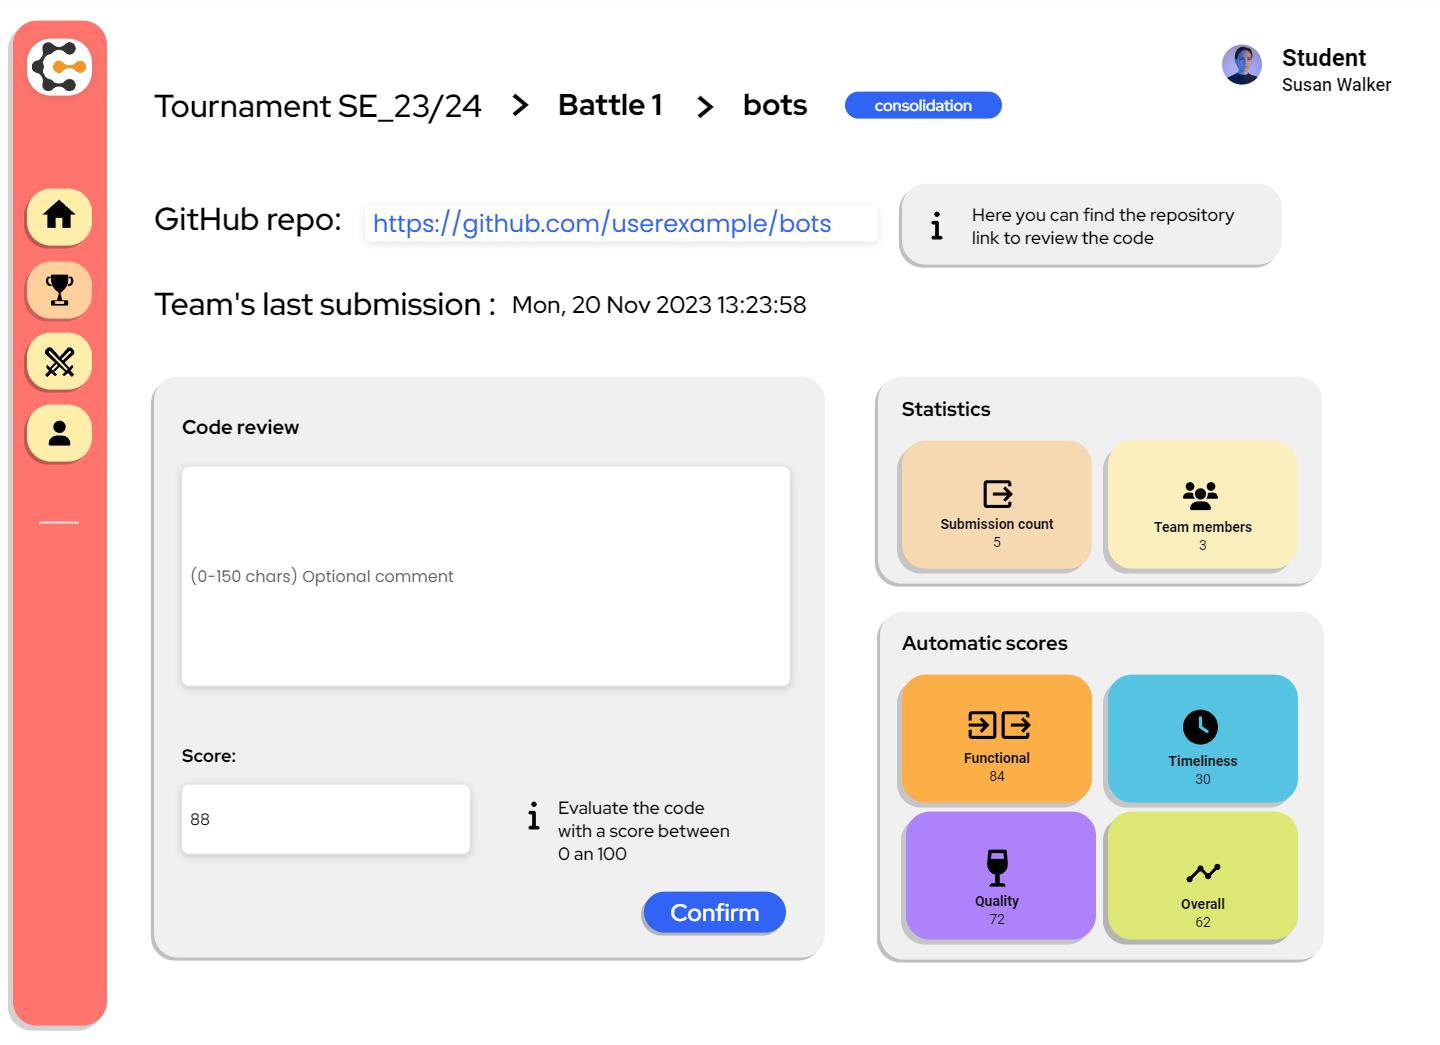
\includegraphics[width=0.8\textwidth]{Mockups/17_educator_manual.png}
        \caption{Page used from Educators to manually evaluate a submission}
    \end{figure}
\end{enumerate}

\subsubsection{Hardware Interfaces}
The software does not require any other hardware interface different than personal computers or smartphones equipped with modern browser from which users can access the platform.
\subsubsection{Software Interfaces}
Some of the functionalities provided by the system exploit specific interfaces to work. These are:
\begin{itemize}
    \item \textbf{GitHub interface}: the system must be able to interface with GitHub API to create the original repository for each battle and to pull code submissions.
    \item \textbf{Static analysis tools}: some of the aspects that have to be evaluated require the execution of some static analysis method over the provided code. In this case, the platform utilizes external services directly provided by third-party organizations.
\end{itemize}
Each of these interfaces are implemented by correctly setting and utilizing specific API calls to the involved services that will be included inside the platform’s inner processes.

Moreover, in order to be notified about the submission of a new solution, the system itself must expose a REST endpoint that will be invoked by the automated GitHub Actions workflow set up by each team on their repository.
\subsubsection{Communication Interfaces}
From the moment that most of the system’s services are provided through the platform’s website and REST API calls, no other protocol than normal HTTP should be needed. Anyway, it is worth mentioning that communication between the system and user is achieved through notifications sent via mail using an external mail service provider.

\subsection{Functional Requirements}
The main requirements the system has to fulfill are the following:
\begin{enumerate}[label=$\bullet$ \textbf{R\arabic*:}]
    \item System shall allow user to register as educator or student.
    \item System shall allow user to log in.
    \item System shall allow educator to create a tournament.
    \item System shall allow educator (tournament creator) to set the name of the tournament.
    \item System shall allow educator (tournament creator) to set the description of the tournament.
    \item System shall allow educator (tournament creator) to set the subscription deadline of the tournament.
    \item System shall notify all students enrolled to the platform about a newly created tournament.
    \item System shall allow educator (tournament creator) to end the tournament.
    \item System shall allow educator (tournament creator) to add another educator as collaborator to the tournament.
    \item System shall allow educator (tournament creator or collaborator) to create a battle for the tournament.
    \item System shall allow educator (tournament creator or collaborator) to upload the Code Kata of the battle.
    \item System shall allow educator (battle creator) to set minimum and maximum number of students per group allowed for the battle.
    \item System shall allow educator (battle creator) to set the registration deadline of the battle.
    \item System shall allow educator (battle creator) to set the submission deadline of the battle.
    \item System shall allow educator (battle creator) to enable/disable optional manual evaluation for the battle.
    \item System shall allow educator (battle creator) to select relevant aspects of code quality to be extracted through static analysis.
    \item System shall notify all users enrolled to a tournament about a newly created battle.
    \item System shall integrate with external static analysis tools through proper API calls.
    \item System shall create the GitHub repository of a battle as soon as the registration phase closes.
    \item System shall assign to each submission sent before the submission deadline a score (natural number between 0 and 100) combining correctness, timeliness and code quality \textit{as soon as possible}.
    \item System shall allow educator (battle creator) to set a manual score (natural number between 0 and 100) to the last valid team’s submission during the consolidation stage of the battle.
    \item System shall compute a final score combining automatic and manual score (if available) for each team after the consolidation stage if expected or after the submission deadline otherwise.
    \item System shall update the battle teams’ ranks right after a new score is available.
    \item System shall notify all students participating to the battle about the availability of the final battle rank.
    \item System shall update the tournament students’ scores as the sum of all the battle scores received during the tournament once the final battle rank becomes available.
    \item System shall notify all involved users about the availability of the tournament student’s final rank.
    \item System shall allow all users to see the list of ongoing tournaments.
    \item System shall allow all users to see all tournaments’ ranks.
    \item System shall allow all users subscribed to the same battle the relative battle's rank.
    \item System should manage every ranking (tournament or battle) in a way that it represents the correct order of students/teams within its context, from the ones with the highest score to the ones with the lowest.
    \item System shall allow student to enroll to a tournament within the subscription deadline.
    \item System shall allow student to create a team within the registration deadline.
    \item System shall allow student (team creator) to set the team name.
    \item System shall allow student (team creator) to set the privacy of the group.
    \item System shall allow student to join a team \textit{only} before the registration deadline.
    \item System shall allow \textit{only} students who know the correct invite code to join private groups.
    \item System shall allow team members to set their the repository URL.
    \item System shall generate a unique API token for each team.
    \item System should offer an external API which, when invoked, will notify the platform about a new commit on a team’s GitHub repository.
\end{enumerate}
\subsubsection{Use cases}
TODO
\subsubsection{Goals mapping}
$\bullet$ \textbf{G1}: Allow students to participate to collaborative programming challenges
\begin{center}
    \begin{tabular}{ |m{3cm}|m{10cm}| }
        \hline
        \textbf{Requirements} 
        & \textbf{R1}: System shall allow user to register as educator or student \\
        & \textbf{R2}: System shall allow user to log in \\
        & \textbf{R7}: System shall notify all students enrolled to the platform about a newly created tournament \\
        & \textbf{R17}: System shall notify all users enrolled to a tournament about a newly created battle \\
        & \textbf{R19}: System shall create the GitHub repository of a battle as soon as the registration phase closes \\
        & \textbf{R27}: System shall allow all users to see the list of ongoing tournaments \\
        & \textbf{R31}: System shall allow student to enroll to a tournament within the subscription deadline \\
        & \textbf{R32}: System shall allow student to create a team within the registration deadline \\
        & \textbf{R33}: System shall allow student (team creator) to set the team name \\
        & \textbf{R34}: System shall allow student (team creator) to set the privacy of the group \\
        & \textbf{R35}: System shall allow student to join a team \textit{only} before the registration deadline \\
        & \textbf{R36}: System shall allow \textit{only} students who know the correct invite code to join private groups \\
        & \textbf{R37}: System shall allow team members to set their the repository URL \\
        & \textbf{R38}: System shall generate a unique API token for each team \\
        & \textbf{R39}: System should offer an external API which, when invoked, will notify the platform about a new commit on a team’s GitHub repository \\
        \hline
    \end{tabular}
    \begin{tabular}{ |m{3cm}|m{10cm}| }
        \hline
        \textbf{Domain \newline Assumptions} 
        & \textbf{D1}: Users have access to a stable and reliable internet connection to interact with the CKB platform \\
        & \textbf{D5}: Students are expected to engage in Code Kata Battles with integrity, without resorting to plagiarism or cheating (e.g. inviting more or different collaborators with respect to the ones inside the team) \\
        & \textbf{D6}: Maximum number of students per group an educator can set will always be bounded (e.g. less than 4) \\
        & \textbf{D7}: Every student has a GitHub account \\
        & \textbf{D8}: Students will fork the Code Kata GitHub repository once ready \\
        & \textbf{D9}: Students know how to setup a GitHub Actions worfkflow \\
        & \textbf{D10}: Only one student per group will perform the steps needed to set-up the team's repository and the GitHub Actions workflow \\
        & \textbf{D12}: Students use external communication channels \\
        \hline
    \end{tabular}
\end{center}
\newpage
$\bullet$ \textbf{G2}: Allow educators to create programming challenges
\begin{center}
    \begin{tabular}{ |m{3cm}|m{10cm}| }
        \hline
        \textbf{Requirements} 
        & \textbf{R1}: System shall allow user to register as educator or student \\
        & \textbf{R2}: System shall allow user to log in \\
        & \textbf{R3}: System shall allow educator to create a tournament \\
        & \textbf{R4}: System shall allow educator (tournament creator) to set the name of the tournament \\
        & \textbf{R5}: System shall allow educator (tournament creator) to set the description of the tournament \\
        & \textbf{R6}: System shall allow educator (tournament creator) to set the subscription deadline of the tournament \\
        & \textbf{R8}: System shall allow educator (tournament creator) to end the tournament \\
        & \textbf{R9}: System shall allow educator (tournament creator) to add another educator as collaborator to the tournament \\
        & \textbf{R10}: System shall allow educator (tournament creator or collaborator) to create a battle for the tournament \\
        & \textbf{R11}: System shall allow educator (tournament creator or collaborator) to upload the Code Kata of the battle \\
        & \textbf{R12}: System shall allow educator (battle creator) to set minimum and maximum number of students per group allowed for the battle \\
        & \textbf{R13}: System shall allow educator (battle creator) to set the registration deadline of the battle \\
        & \textbf{R14}: System shall allow educator (battle creator) to set the submission deadline of the battle \\
        & \textbf{R15}: System shall allow educator (battle creator) to enable/disable optional manual evaluation for the battle \\
        & \textbf{R16}: System shall allow educator (battle creator) to select relevant aspects of code quality to be extracted through static analysis \\
        \hline
    \end{tabular}
    \begin{tabular}{ |m{3cm}|m{10cm}| }
        \hline
        \textbf{Domain \newline Assumptions} 
        & \textbf{D1}: Users have access to a stable and reliable internet connection to interact with the CKB platform \\
        & \textbf{D2}: Supported programming languages are limited to popular options like Java, Python and C++ \\
        & \textbf{D3}: Registered educators are all legitimate and verified \\
        & \textbf{D4}: Educators upload correct test cases and well-structured Code Kata projects \\
        & \textbf{D6}: Maximum number of students per group an educator can set will always be bounded (e.g. less than 4) \\
        \hline
    \end{tabular}
\end{center}        
$\bullet$ \textbf{G3}: Allow the system to automatically evaluate students' submissions
\begin{center}
    \begin{tabular}{ |m{3cm}|m{10cm}| }
        \hline
        \textbf{Requirements} 
        & \textbf{R18}: System shall integrate with external static analysis tools through proper API calls \\
        & \textbf{R19}: System shall create the GitHub repository of a battle as soon as the registration phase closes \\
        & \textbf{R20}: System shall assign to each submission sent before the submission deadline a score (natural number between 0 and 100) combining correctness, timeliness and code quality \textit{as soon as possible} \\
        & \textbf{R22}: System shall compute a final score combining automatic and manual score (if available) for each team after the consolidation stage if expected or after the submission deadline otherwise \\
        & \textbf{R37}: System shall allow team members to set their the repository URL \\
        & \textbf{R38}: System shall generate a unique API token for each team \\
        & \textbf{R39}: System should offer an external API which, when invoked, will notify the platform about a new commit on a team’s GitHub repository \\
        \hline
    \end{tabular}
    \begin{tabular}{ |m{3cm}|m{10cm}| }
        \hline
        \textbf{Domain \newline Assumptions} 
        & \textbf{D2}: Supported programming languages are limited to popular options like Java, Python and C++ \\
        & \textbf{D4}: Educators upload correct test cases and well-structured Code Kata projects \\
        & \textbf{D8}: Students will fork the Code Kata GitHub repository once ready \\
        & \textbf{D9}: Students know how to setup a GitHub Actions worfkflow \\
        & \textbf{D10}: Only one student per group will perform the steps needed to set-up the team's repository and the GitHub Actions workflow \\
        & \textbf{D11}: Static analysis tools are able to quantify the specified code quality aspects \\
        \hline
    \end{tabular}
\end{center} 
$\bullet$ \textbf{G4}: Allow educators to manually evaluate students' submissions
\begin{center}
    \begin{tabular}{ |m{3cm}|m{10cm}| }
        \hline
        \textbf{Requirements} 
        & \textbf{R1}: System shall allow user to register as educator or student \\
        & \textbf{R2}: System shall allow user to log in \\
        & \textbf{R14}: System shall allow educator (battle creator) to set the submission deadline of the battle \\
        & \textbf{R15}: System shall allow educator (battle creator) to enable/disable optional manual evaluation for the battle \\
        & \textbf{R21}: System shall allow educator (battle creator) to set a manual score (natural number between 0 and 100) to the last valid team’s submission during the consolidation stage of the battle \\
        \hline
        \textbf{Domain \newline Assumptions} 
        & \textbf{D1}: Users have access to a stable and reliable internet connection to interact with the CKB platform \\
        & \textbf{D8}: Students will fork the Code Kata GitHub repository once ready \\
        & \textbf{D10}: Only one student per group will perform the steps needed to set-up the team's repository and the GitHub Actions workflow \\
        \hline
    \end{tabular}
\end{center} 
\newpage
$\bullet$ \textbf{G5}: Allow students to track their performance
\begin{center}
    \begin{tabular}{ |m{3cm}|m{10cm}| }
        \hline
        \textbf{Requirements} 
        & \textbf{R1}: System shall allow user to register as educator or student \\
        & \textbf{R2}: System shall allow user to log in \\
        & \textbf{R18}: System shall integrate with external static analysis tools through proper API calls \\
        & \textbf{R20}: System shall assign to each submission sent before the submission deadline a score (natural number between 0 and 100) combining correctness, timeliness and code quality \textit{as soon as possible} \\
        & \textbf{R21}: System shall allow educator (battle creator) to set a manual score (natural number between 0 and 100) to the last valid team’s submission during the consolidation stage of the battle \\
        & \textbf{R22}: System shall compute a final score combining automatic and manual score (if available) for each team after the consolidation stage if expected or after the submission deadline otherwise \\
        & \textbf{R23}: System shall update the battle teams’ ranks right after a new score is available \\
        & \textbf{R24}: System shall notify all students participating to the battle about the availability of the final battle rank \\
        & \textbf{R25}: System shall update the tournament students’ scores as the sum of all the battle scores received during the tournament once the final battle rank becomes available \\
        & \textbf{R26}: System shall notify all involved users about the availability of the tournament student’s final rank \\
        & \textbf{R28}: System shall allow all users to see all tournaments’ ranks \\
        & \textbf{R29}: System shall allow all users subscribed to the same battle the relative battle's rank \\
        & \textbf{R30}: System should manage every ranking (tournament or battle) in a way that it represents the correct order of students/teams within its context, from the ones with the highest score to the ones with the lowest \\    
        \hline
    \end{tabular}
    \begin{tabular}{ |m{3cm}|m{10cm}| }
        \hline
        \textbf{Domain \newline Assumptions} 
        & \textbf{D1}: Users have access to a stable and reliable internet connection to interact with the CKB platform \\
        \hline
    \end{tabular}
\end{center} 

\subsection{Performance Requirements}
Even though the platform is not mission critical, should guarantee a smooth and appealing experience to all kind of users. Given the complexity of the overall project, we describe different performance requirements for different aspects:
\begin{itemize}
    \item \textit{Basic user interaction with the webapp}: response time for user actions like creating/joining a team, loading scoreboards, creating a tournament etc should be under 2 seconds for 90\% of requests under normal load.
    \item \textit{Space requirements}: a reasonable estimate of a project’s maximum size is about 40-50 MB. So, the system, to control the space usage, should limit the allowed projects sizes to 80 MB.
    \item \textit{Upload/download speed requirements}: given the previous estimate of project’s size, the system should guarantee a good throughput in terms of upload and download speed of the projects’ files. System should be able to reserve on average at least 8 Mb/s to each connection; this means that a project directory of 50 MB would take about 50 seconds to be downloaded. However, bandwidth of educator’s uploads should be prioritized. A pessimistic estimate with 1000 concurrent upload/download connections suggests that the systems needs at least a 10 Gb/s internet connection. Aggregating different Internet Service Providers may be considered to achieve greater bandwidths.
    \item \textit{Computational resources}: system should be sized to handle up to 100 simultaneous code submissions from different teams, providing a score within 20 seconds. Multiple CPUs with worker pooling approach will help in handling this kind of concurrency, dealing also with scalability issues.
    \item \textit{Notifications}: email notification should be able to reach all the recipients within 2 minutes.
\end{itemize}
These performance requirements will be taken in consideration also in choosing the external static analysis provider.

Moreover, given the different and independent performance requirements of all the functions involved, it is preferred to support each one with different machines or subsystems. In this way, the overall platform could still work with degraded performance affecting only a part of the functionalities.

The performance of the system could be improved following some basic strategies:
\begin{itemize}
    \item \textbf{Limit inbound API rate}: this will help in reducing commits from the same team (preventing also spam attacks).
    \item \textbf{Bound execution time}: terminate the evaluation of a submission after a timeout. This will help to prevent excessive resource consumption on tasks that should be quick to perform. 
\end{itemize}
In conclusion, it is important to mention again that even though the system is not providing an essential service to the user, it should offer a non stressful educational experience. Indeed, given the strict deadlines system, even a little delay in the submission can compromise the competition (which could potentially reflect into school marks of students), thus the overall purpose of the project.

\subsection{Design Constraints}
\subsubsection{Standards compliance}
There are several standards the system must comply with:
\begin{itemize}
    \item The web interface will comply with the latest versions of HTML, CSS and JavaScript standards.
    \item API will follow REST architectural constraints and use JSON data formats.
    \item Coordinated Universal Time (UTC) will be used to store timestamps in order to correctly show deadlines to user located in different time-zones.
\end{itemize}
\subsubsection{Hardware limitations}
The CDK platform has no strict hardware requirements, but should perform well on average smartphone or computer equipped with a modern web browser and a reliable internet connection.
\subsubsection{Privacy constraints}
Since the platform will need to ask the user for personal information like name, surname and email address, it needs to guarantee that this data will be processed and stored accordingly to the GDPR. Moreover, from the moment that the platform will also use cookies (e.g. to keep users authenticated), the system will need to get consent from visitors before placing cookies on their devices, in compliance with the EU ePrivacy regulations.
\subsubsection{Quality constraints}
User acceptance testing will measure task success rate and user satisfaction.

\subsection{Software System Attributes}
\subsubsection{Reliability}
Given the complexity of the project, reaching high reliability levels represents a challenge and a key to success for the product. Indeed, even though the systems performs many interactions with external actors and service providers, consistency and integrity of the overall platform should be guaranteed even in case of errors or unexpected conditions.
\subsubsection{Availability}
Service should be continuously available (24/7) to users, with little downtime and rapid service recovery. The overall service level target is 99.5\%, which corresponds nearly to 50 minutes of downtime per week. Planned maintenances should be communicated to users in advance, given the strict time requirements of the service offered by the platform.
\subsubsection{Usability}
The platform should be intuitive and minimal, still offering all the functionalities needed by all kind of users.
\subsubsection{Security}
\begin{itemize}
    \item Passwords must be securely hashed and salted before storage.
    \item Encryption should be used for sensitive data.
    \item Input validation and sanitization should be applied to prevent attacks.
    \item Adopt HTTPS protocol, which uses encryption for secure communication.
    \item Deploy firewalls to protect the system from unauthorized access.
    \item Employ API authentication mechanism to limit access to the API.
\end{itemize}
\subsubsection{Scalability}
The system should be designed to easily scale horizontally to accommodate growth in traffic.

%------------------------------------------------------------------------------------------------------------------------------------------------
\clearpage
{\color{Blue}{\section{Formal Analysis Using Alloy}}}
\label{sect:alloy}
An Alloy model is provided to present a formal description of the system. 
The goals of this kind of analysis are to check the consistency of the model and to find possible errors and corner cases in the requirements.\\
A formal model is also useful to express complex facts which are not captured by the domain class diagram such as the constraints involving subcriptions, scores, timestamps, battle and tournament states.\\ \\

\subsection{Model Code}
\begin{lstlisting}[language=alloy]
open util/integer

//SIGNATURES

sig Email {}

sig Password {}

sig GithubUsername {}

abstract sig User {

    email: Email,

    password: Password

}

sig Student extends User {

    username: one GithubUsername

}

sig Educator extends User {

    createsTournament: set Tournament,

    createBattle: set Battle

}






sig Timestamp {

    time: Int

} { 
    time >= 0 
}

one sig SystemTimestamp {

    ts: Timestamp

}

pred earlierThan [t1, t2: Timestamp] {

    int t1.time < int t2.time

}

pred earlierEqual [t1, t2: Timestamp] {

    int t1.time <= int t2.time

}

enum TournamentState { Subscription, Ongoing, Ended }

sig Tournament {

    subscriptionDeadline: Timestamp,

    state: TournamentState ,

    isManaged: some Educator,

    battles: set Battle,

    participants: set Student -> one Score

}

sig TestCase {}

sig CodeKata {

testCases: some TestCase

}

enum Bool { True, False }

enum ProgrammingLanguage { Python, Java, C }

enum BattleState { TeamFormation, SubmissionPhase, ConsolidationPhase, Finished }

sig Battle {

    state: BattleState ,

    participants: set Team,

    registrationDeadline: Timestamp,

    submissionDeadline: Timestamp,

    minTeamSize: Int,

    maxTeamSize: Int,

    programmingLanguage: ProgrammingLanguage,

    codeKata: CodeKata,

    a1Eval: Bool,

    a2Eval: Bool,

    a3Eval: Bool,

    manualEval: Bool

}  {

    earlierThan[registrationDeadline,submissionDeadline]

    minTeamSize > 0

    maxTeamSize >= minTeamSize

}

sig Score {

    value: Int

} {

    int value >= 0

}

sig Submission {

    ts: one Timestamp,

    functionalScore: one Score,

    timelinessScore: one Score,

    a1Score: lone Score,

    a2Score: lone Score,

    a3Score: lone Score,

    qualityScore: one Score,

    manualScore: lone Score,

    overallScore: one Score,

    battle: Battle

}

sig ApiToken{}

sig InviteCode{}

sig Team {

    submissions: set Submission,

    participates: one Battle,

    members: some Student,

    battleScore: one Score,

    apiToken: one ApiToken,

    inviteCode: one InviteCode

}


//INTEGRITY CONSTRAINTS

// each password is associated to some user ( some registration may have the same password )
fact eachPasswordToSomeUser{
all p : Password | ( some u : User | u. password = p)
}

// each Int associated to at most 1 timestamp
fact oneTimestampPerInteger{
all i:Int | ( lone t : Timestamp | t.time = i)
}

// each Intt associated to at most 1 score
fact oneTimestampPerInteger{
all i:Int | ( lone s : Score | s.value = i)
}

// each username is associated to a unique student
fact eachGitHubUsernameToOneStudent{
all u : GithubUsername | ( one s : Student | s. username = u)
}

// each ApiToken is associated to a unique team
fact eachApitTokenToOneTeam{
all a : ApiToken | ( one t : Team | t. apiToken= a)
}

// each InviteCode is associated to a unique team
fact eachInviteCodeToOneTeam{
all i : InviteCode | ( one t : Team | t. inviteCode= i)
}

// each email is associated to a unique user 
fact eachEmailToOneUser{
all e : Email| ( one u : User | u. email= e)
}

// each tournament has 1 creator
fact eachTournamentHasOneCreator{
all t : Tournament | ( one e : Educator | t in e.createsTournament )
}

// each battle has 1 creator
fact eachBattleHasOneCreator{
all b : Battle | ( one e : Educator | b in e.createBattle)
}

// each battle belongs to only a tournament
fact eachBattleToOneTournament{
all b: Battle| (one t : Tournament | b in t.battles )
}

// each testcase belongs to only a code kata
fact eachTestCaseToOneCodeKata{
all t: TestCase| (one c : CodeKata| t in c.testCases )
}

// each CodeKata belongs to only a battle
fact eachCodeKataToOneBattle{
all c: CodeKata| (one b : Battle| c in b.codeKata )
}

// each Submission belongs to only a Team
fact eachSubmissionToOneTeam{
all s: Submission| (one t : Team| s in t.submissions )
}

// coherence between battle's participants and team's participates
fact coherenceBetweenParticipantsAndParticipate{
all t: Team, b: Battle | t in b.participants <==> t.participates = b
}








//ADDITIONAL CONSTRAINTS

//tournament is on ongoing state if and only if subscription deadline has elapsed
fact tournamentStateCoherentWithSystemTimestamp{
all t:Tournament | earlierThan[t.subscriptionDeadline, SystemTimestamp.ts] <=> t.state = Ongoing
}

// battle states coherent with system timestamp
fact battleStateCoherentWithSystemTimestamp{
all b:Battle | 
    (earlierThan[SystemTimestamp.ts, b.registrationDeadline] 
        implies b.state = TeamFormation) and
    ((earlierEqual[ b.registrationDeadline,SystemTimestamp.ts] and earlierThan[ SystemTimestamp.ts, b.submissionDeadline]) 
        implies b.state = SubmissionPhase) and
    (earlierEqual[ b.submissionDeadline,SystemTimestamp.ts] 
        implies (b.state = ConsolidationPhase or b.state = Finished) )
}

//submission ts come before system timestamp
fact submissionTsBeforeSystemTimestamp{
all s:Submission | earlierEqual[s.ts, SystemTimestamp.ts]
}

// each student can subscribe only once to a tournament
fact eachStudentSubscribesMostOnce{
all t:Tournament, s:Student | #t.participants[s] <= 1
}

// tournament creator is also managing the tournament (tournament has at least 1 educator managing it)
fact creatorCanManage{ 
all e: Educator, t:e.createsTournament  | e in t.isManaged 
}

// tournament's participants scores are the sum of battle scores obtained by the teams the student is a member of in the battles of that tournament
fun allStudentTeamsInEndedBattles[s:Student]:set Team{
{t:Team | s in t.members and t.participates.state = Finished}
}
fun totalTournamentScore[t: Tournament, s: Student]: Int {
sum te: t.battles.participants&allStudentTeamsInEndedBattles[s] | int te.battleScore.value
}
fact TournamentParticipantsScoreComputation{ 
all t: Tournament, s: Student | #t.participants[s] = 1 implies int t.participants[s].value = int totalTournamentScore[t,s]
}

// submission's quality score is the sum of all aspects scores
fun add3Scores[a, b, c: Score]: Score {
{i: Score | int i.value = integer/add[ integer/add[a.value, b.value], c.value]}
}
fact qualityScoreCombinesAspectsScores {
all s:Submission | s.qualityScore = add3Scores[s.a1Score, s.a2Score, s.a3Score] 
}

// submission's overall score is the sum of all the scores
fun add4Scores[a, b, c, d: Score]: Score {
{i: Score | int i.value = integer/add[integer/add[integer/add[a.value,b.value],c.value], d.value]}
}
fact OverallScoreCombinesAutoAndManualScore {
all s:Submission | s.overallScore = add4Scores[s.functionalScore, s.timelinessScore, s.qualityScore, s.manualScore]
}

// battleScore is the overall score of the team's last submission
fun lastSubmission[t: Team]: one Submission {
{ s: t.submissions | no su: t.submissions - s | earlierThan[s.ts,su.ts] }
}
fact battleScoreIsLastOverallScore {
all t: Team | (#t.submissions= 0 implies int t.battleScore.value = 0) and
	      (#t.submissions >0 implies int t.battleScore.value = int lastSubmission[t].overallScore.value)
}

// battle registration deadline comes after tournament subscription deadline
fact RegistrationAfterSubscription {
all b:Battle,to:Tournament | b in to.battles implies earlierThan[to.subscriptionDeadline,b.registrationDeadline]
}

// Student participates only to battles that belong to tournaments he is enrolled in
fact OnlyBattlesInEnrolledTournament {
all s:Student, te:Team, to:Tournament | (s in te.members and te.participates in to.battles) implies (#to.participants[s] = 1)
}

// a battle can be associated to a tournament only if the tournament is not in registration phase anymore
fact NoBattleInTournamentSubscription {
no t:Tournament | t.state = Subscription and #t.battles > 0
}

// if a tournament is ended, then all its battles must be ended too
fact AllBattleEndedIfTournamentEnded {
all t:Tournament| t.state = Ended implies (all b: t.battles | b.state = Finished)
}

// if a battle is in teamFormation/submission/consolidation state, then its tournament must be on ongoing state
fact TournamentOngoingIfBattleNotEnded {
all t:Tournament, b:t.battles | b.state != Finished implies (t.state != Ended)
}

// automated scores of the submission are present only if they are enabled in the battle
fact AutomatedScorePresentIfEnabled {
all s:Submission | (#s.a1Score = 1 <==> s.battle.a1Eval = True) and
		   (#s.a2Score = 1 <==> s.battle.a2Eval = True) and
		   (#s.a3Score = 1 <==> s.battle.a3Eval = True) 
}

// a submission can be associated to a battle only if the battle is in the submission/consolidation/ended state 
fact noSubmissionInTeamFormationPhase {
no s:Submission | s.battle.state = TeamFormation
}

// a submission can happen only after the registration deadline and before the battle's submission deadline
fact SubmissionInSubmissionPhase {
all s:Submission | earlierThan[s.battle.registrationDeadline,s.ts] and earlierThan[s.ts,s.battle.submissionDeadline]
}

// a submission to a battle can occur only if the team is participating to the battle
fact TeamSubmitsOnlyToCorrectBattle {
all t:Team, s:Submission | (s in t.submissions) implies (s.battle = t.participates)
}

// a battle can be created only by educators managing the tournament the battle belongs to
fact BattleCreatedByManager {
all b:Battle, e:Educator, t:Tournament | (b in e.createBattle and b in t.battles) implies (e in t.isManaged)
}

// team members count respects battle's settings
fact TeamSize {
all t:Team | #t.members >= int t.participates.minTeamSize and
	     #t.members <= int t.participates.maxTeamSize
}

// a student can participate to a battle only with 1 team
fact OnlyOneTeamPerBattle {
no t1,t2:Team,s:Student  | t1 != t2 and
			   s in t1.members and
			   s in t2.members and
			   t1.participates = t2.participates
}

// tournament scores initialized to 0  (if tournament is not started yet or none of its battles are ended)
fact ZeroInitializedTournamentScores {
all s:Student, to:Tournament, b:Battle | (#to.participants[s] = 1 
	and (to.state = Subscription or (b in to.battles and b.state != Finished) ) ) implies to.participants[s].value = 0
}

// if a submission comes after another, then its timeliness score should be lower
fact LowerTimelinessScore {
all b:Battle, disj s1,s2:Submission  |  (b in s1.battle and b in s2.battle and earlierThan[s1.ts,s2.ts]) 
    	implies 
    int s1.timelinessScore.value > int s2.timelinessScore.value
}

// There no exist 2 concurrent submissions from same team
fact NoConcurrentSubmission{
all t:Team| no disj s1,s2:t.submissions  |  s1.ts.time = s2.ts.time
}

// a student can be enrolled to a tournament at most once
fact NoDoubleEnrollment {
no to:Tournament, s:Student| #to.participants[s] > 1 
}

// a battle can enter ConsolidationPhase only if manual evaluation is enabled
fact consolidationPhaseOnlyWithManualEval{
all b: Battle | b.state = ConsolidationPhase implies b.manualEval = True
}

// manual score can be present only if the related battle is in consolidation phase or finished
fact ManualScoreOnlyInConsolidationOrFinished{
all s: Submission | #s.manualScore = 1 implies (s.battle.state = ConsolidationPhase or s.battle.state = Finished)
}

// manual score in the submission is present only if its enabled in the battle
fact ManualScorePresentIfEanbled {
all s:Submission | #s.manualScore = 1 implies s.battle.manualEval = True 
}

// manualScore can be present only in the last submission
fact manualScoreOnlyInLastSubmission{
all t: Team, s: t.submissions | #s.manualScore = 1 implies s = lastSubmission[t]
}

// if a battle is ended, manualScore must be present in the last submission
fact manualScoreWhenBattleFinished{
all t: Team | (t.participates.state = Finished and t.participates.manualEval = True) 
        implies 
    #lastSubmission[t].manualScore = 1
}






// Show predicates
pred world1{
#Tournament=1
#Educator=2
#Battle=2
#Tournament.isManaged=2
}

pred world2{
#Tournament=1
#Educator=1
#Battle=2
#Team=2
#Submission=3
}

run world1  for 6
\end{lstlisting}

\subsection{Static analysis}
\begin{lstlisting}[language=alloy]
//Check that all students enrolled in the tournament have 0 tournament score during subcription phase
assert StudentTournamentScoreBeforeStart{
    all t : Tournament, s:Student | (#t.participants[s]=1 and t.state=Subscription) implies int t.participants[s].value = 0
}
check StudentTournamentScoreBeforeStart for 4

//Check that all students enrolled to tournament without any finished battle have 0 tournament score
assert StudentTournamentScoreNoFinishedBattles{
    all t : Tournament, s:Student|(#t.participants[s]=1 and t.state=Ongoing and (no b: t.battles, te:b.participants |  b.state = Finished and s in te.members)) implies int t.participants[s].value = 0
}
check StudentTournamentScoreNoFinishedBattles for 4

//Check that all students enrolled to tournament with a tournament score greater than 0 have participated to at least 1 finished battle in that tournament
assert StudentParticipatesWithTeam{
    all t : Tournament, s:Student| int t.participants[s].value > 0 implies ( some b:t.battles,te:t.battles.participants | b.state=Finished and s in te.members)
}
check StudentParticipatesWithTeam for 4

//Check that all teams enrolled to the battle have 0 battle score before their first submission
assert TeamScoreZeroBeforeSubmissions{
    all b : Battle, te:b.participants | (#te.submissions = 0) implies int te.battleScore.value = 0
}
check TeamScoreZeroBeforeSubmissions for 4

//Check that all teams having battle score greater than 0 have at least 1 submission
assert TeamNonZeroScore{
    all b : Battle, te:b.participants |  int te.battleScore.value > 0  implies  (#te.submissions > 0)
}
check TeamNonZeroScore for 4

//Check that all teams's latest submission have been manually evaluated if a battle is ended
assert AllTeamsManuallyEvaluated{
    no b : Battle |  b.manualEval = True and b.state=Finished and (some te:b.participants | #lastSubmission[te].manualScore = 0)
}
check AllTeamsManuallyEvaluated for 4

\end{lstlisting}
\hfill \break
The alloy model previously presented focuses on the most important entities and attributes of the domain, which are strictly necessary to describe the main functionalities of the system. Indeed, some concepts such as time and scores have been simplified to be easily handled by the Alloy Analyzer and syntax.\\
Images of three world examples are shown below, the first focuses on educators, tournaments and battles, while the second and the third ones include all the aspects related to students, teams and submissions.
\newpage

\begin{figure}[H]
    \vspace{-2cm}
    \hspace{-4cm}
    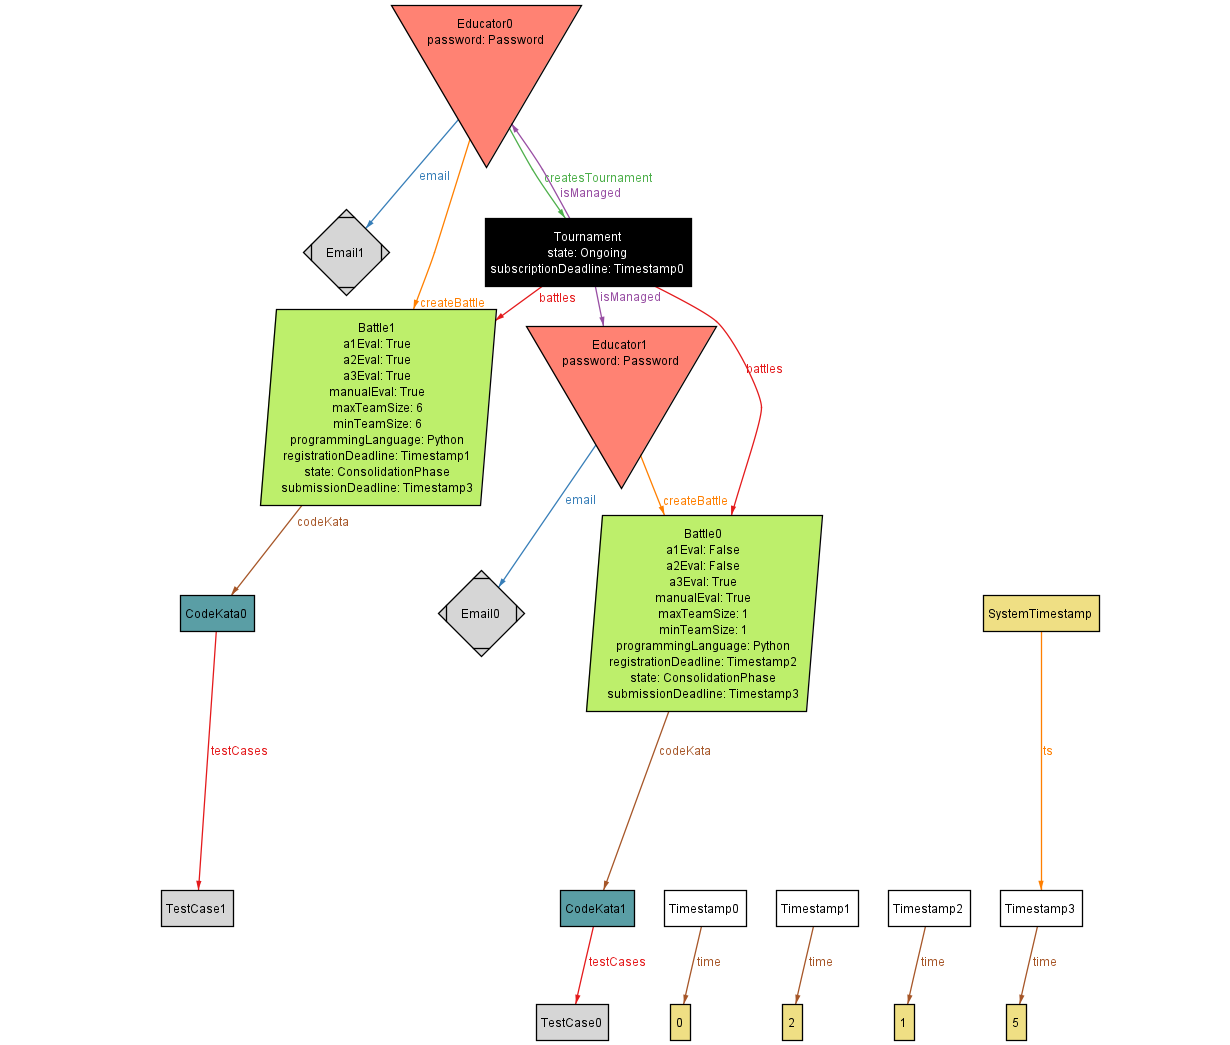
\includegraphics[width=1.65\textwidth]{Alloy/world1.png}
    \vspace{0.2cm}
    \caption{World1, generated with the \textit{world1} predicate}
\end{figure}
\newpage
\begin{figure}[H]
    \centering
    \vspace{-4cm}
    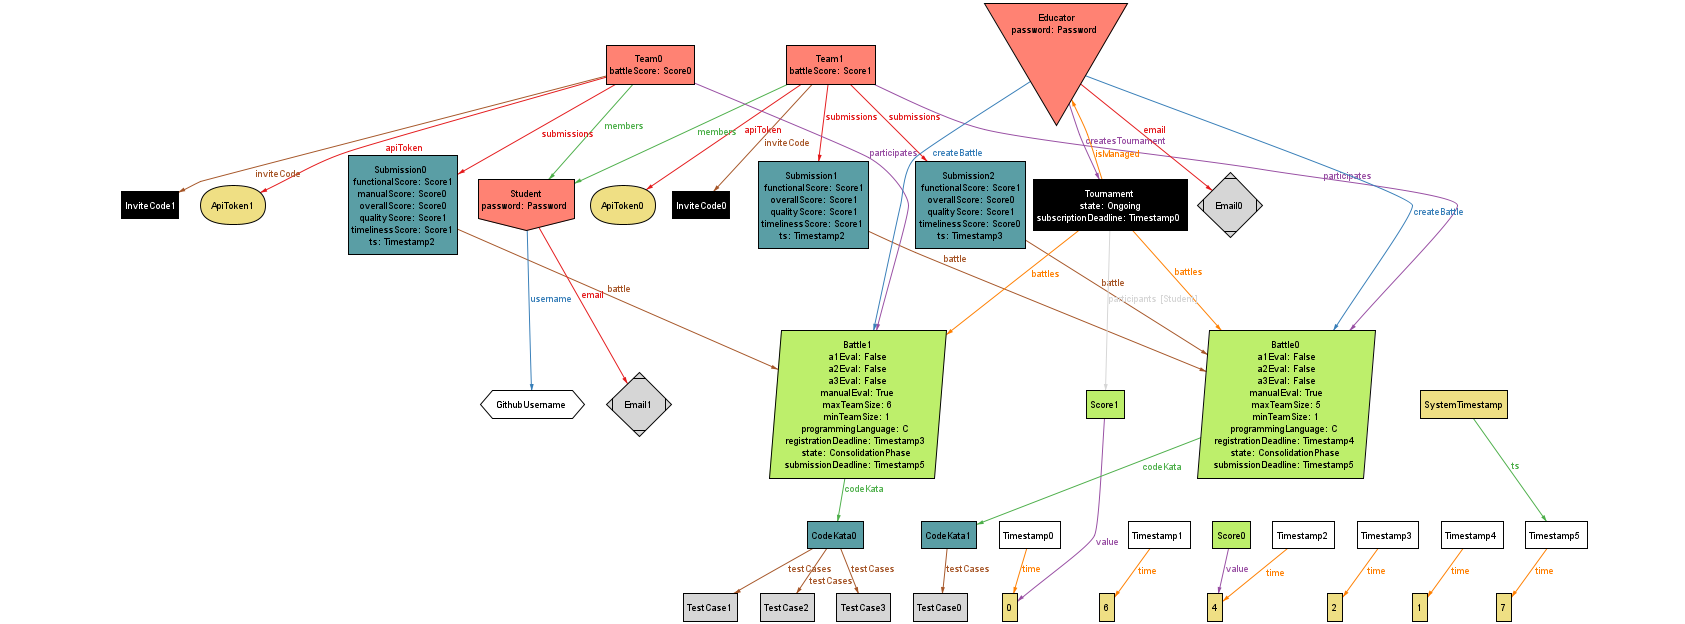
\includegraphics[width=1.65\textwidth,angle=90,origin=c]{Alloy/world2.png}
    \caption{World2, generated with the \textit{world2} predicate}
\end{figure}
\newpage
\begin{figure}[H]
    \centering
    \vspace{-4cm}
    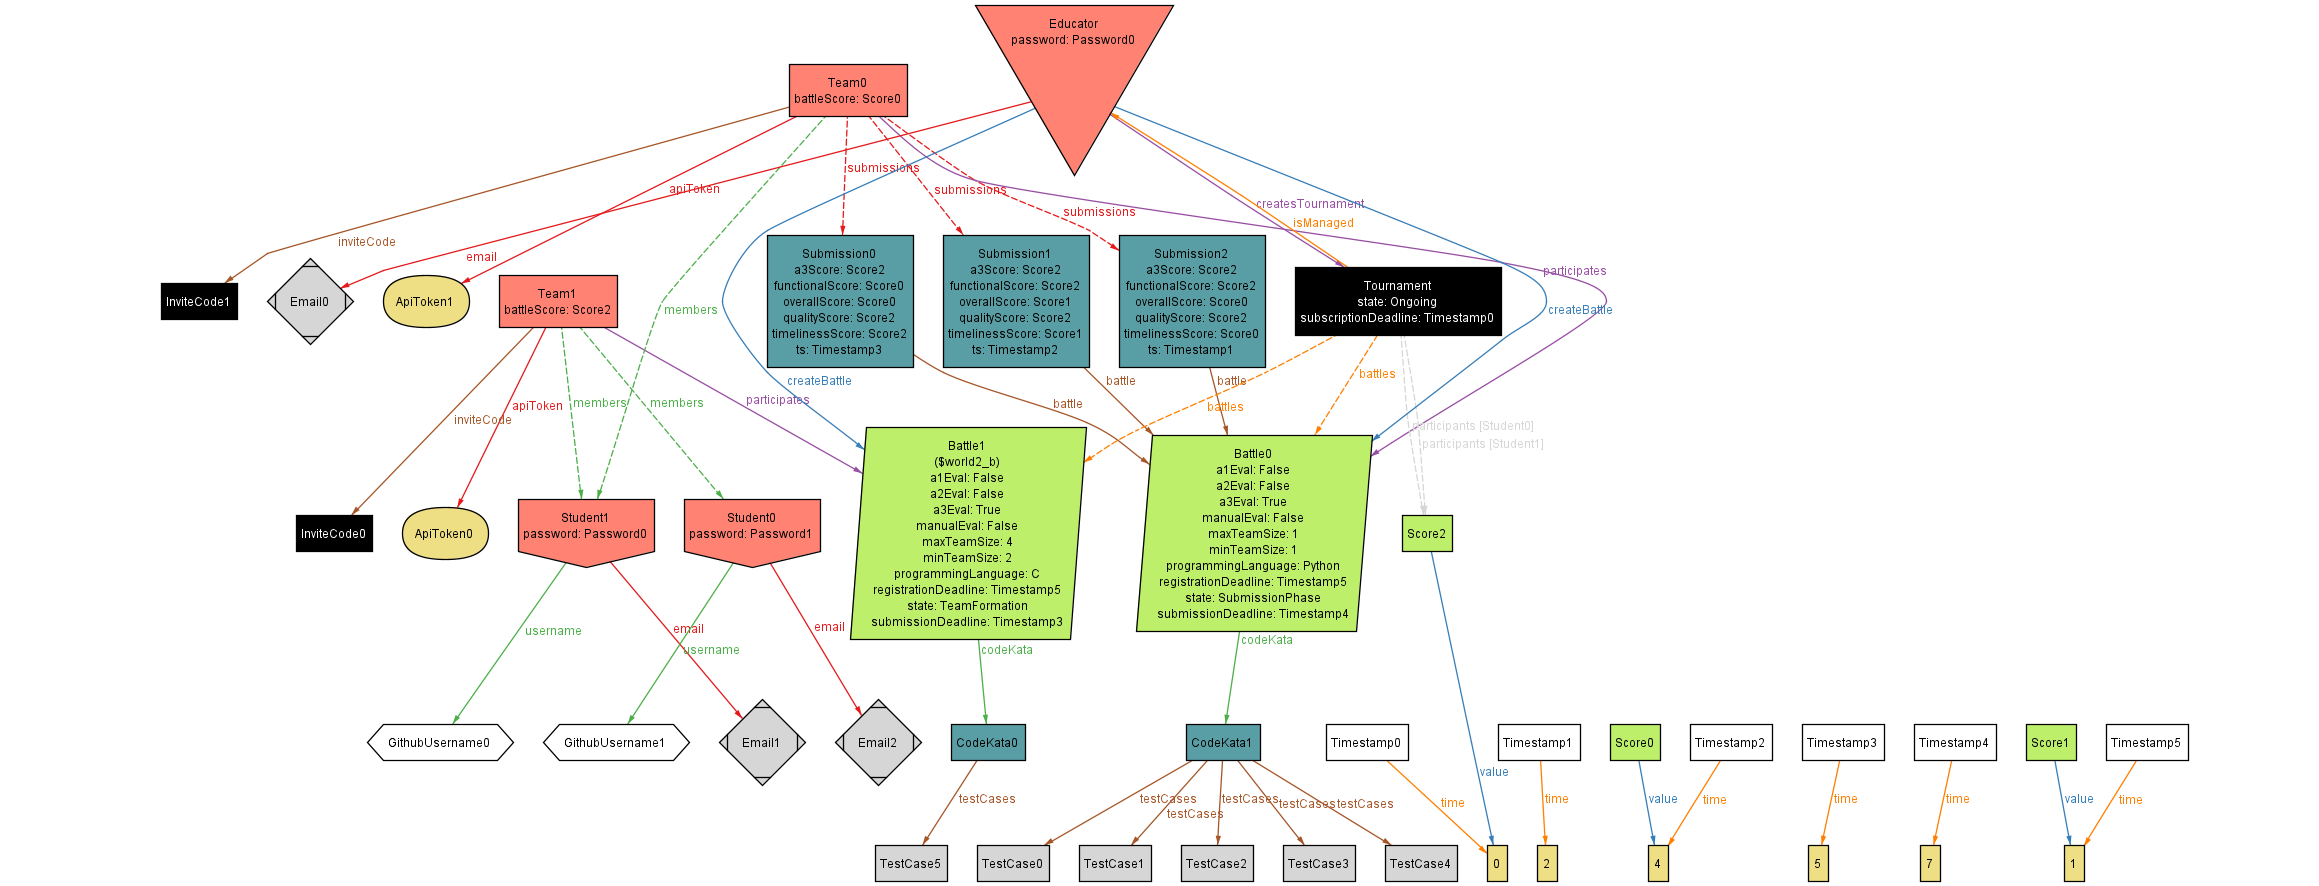
\includegraphics[width=1.65\textwidth,angle=90,origin=c]{Alloy/world3.png}
    \caption{World2, generated with the \textit{world2} predicate}
\end{figure}
\newpage

%------------------------------------------------------------------------------------------------------------------------------------------------
\clearpage
{\color{Blue}{\section{Effort Spent}}}
\label{sect:effort}
\begin{tabular}{|c|c|c|c|c|}
    \hline
    \textbf{Name and Surname} & \textbf{Section 1} & \textbf{Section 2} & \textbf{Section 3} & \textbf{Section 4} \\
    \hline
    Tommaso Capacci & 10 & 10 & 10 & 10 \\
    \hline
    Gabriele Ginestroni & 10 & 10 & 10 & 10 \\
    \hline
\end{tabular}


%------------------------------------------------------------------------------------------------------------------------------------------------
\clearpage
\addcontentsline{toc}{section}{References}
\bibliographystyle{plain}
\bibliography{main}
%------------------------------------------------------------------------------------------------------------------------------------------------




\end{document}
